\documentclass[]{project_report}
\usepackage[hidelinks ]{hyperref}
\usepackage{hyperref}
\usepackage{graphicx}
\usepackage{url} 
\graphicspath{ {images/} }
\usepackage{listings}
\usepackage{xcolor}

\usepackage{minted}
\usepackage{xcolor}
\usepackage{caption}

\DeclareCaptionType{codeblock}[CodeBlock][List of Code Blocks]

\setminted{
    bgcolor=lightgray!20, 
    fontsize=\footnotesize,
    fontfamily=tt,         
    frame=lines,           
    breaklines=true,    
    linenos=true,      
    numbersep=5pt,
}

\usemintedstyle{friendly}


%%%%%%%%%%%%%%%%%%%%%%
%%% Input project details
\def\studentname{Edward Instance}
\def\reportyear{2024}
\def\projecttitle{Advanced Web Development}
\def\supervisorname{Christos Dexiades}
\def\degree{BSc in Computer Science}
\def\fullOrHalfUnit{Full Unit}
\def\finalOrInterim{Final} % indicate if this document is your Final Report or Interim Report

\begin{document}

\maketitle

%%%%%%%%%%%%%%%%%%%%%%
%%% Declaration

\chapter*{Declaration}

This report has been prepared on the basis of my own work. Where other published and unpublished source materials have been used, these have been acknowledged.

\vskip3em

Word Count: 14,760

\vskip3em

Student Name: \studentname

\vskip3em

Date of Submission: 24/4/2025

\vskip3em

Signature: einstance

\newpage

%%%%%%%%%%%%%%%%%%%%%%
%%% Table of Contents
\tableofcontents\pdfbookmark[0]{Table of Contents}{toc}\newpage

%%%%%%%%%%%%%%%%%%%%%%
%%% Your Abstract here
\chapter*{Abstract}
\addcontentsline{toc}{chapter}{Abstract}

Online shopping has become an integral part of everyday life, with over 50 million users in the UK this year alone. This number is projected to rise by more than 10 million in the next five years \cite{amazon_competition}. Most online stores charge transaction fees for sales made on their platforms. For example, Amazon profits from transactions between third-party sellers and users \cite{ecommerce_users}. This project aims to use the demand of online shopping while also prioritising users by removing transaction fees and focusing on a subscription based approach.

This will benefit both buyers and sellers across a wide range of needs and scales. Sellers will avoid high transaction fees and have more predictable costs with the subscription model, as well as being able to scale their subscription based on their usage. Buyers will also benefit from this as items will be cheaper as no one has to pay fees on each item.

This report outlines the application's aims and goals, detailing how it addresses the current challenges of online shopping platforms. There is a focus on the technologies, frameworks, and platforms used, as well as the architectural paradigms and design patterns implemented to build a robust, scalable, and secure application. Further discussion highlights the state-of-the-art approaches employed, including considerations of security, privacy, cloud deployments, and DevOps practices. As well as the focus into what was done to create the project there are also sections on the underpinning software engineering principles that shaped the development and the issues that the project faced throughout its development. 

Finally the report will contain a user manual so that anyone can pickup the project and start using it either locally for development or globally as it is intended, but also so that stakeholders can gain an understanding of the platform without having required technical knowledge.

\chapter{Introduction}

The introduction of this report will cover both an introduction to this report but also to the project as a whole. This report is for summing up the project but to also explain decisions behind it. Firstly you will be introduced to the problem that this project is trying to solve and then how it is going to achieve that though a series of goals and achievements. Then the report describes the technical decisions that were made and the technologies used, as well as the software engineering processes that overarched these. Finally, the report will contain a user manual and a report on the professional issues faced.

There were some constraints to the project that are discussed in the relevant sections, examples of this would be one of the architectural paradigms that has to be used and one of the platforms that must be used.


\section{The problem}

The problem this application is trying to solve is the that selling items online is expensive and unnecessary fees are being added so that platforms can make better margins. While these fees are lucrative for the platform, they significantly reduce profit margins for sellers, particularly small-scale vendors with already tight margins, making it potentially detrimental. Large sellers are also effected by this as they could be losing up to 5\% of their profits per item from fees and this adds up once at a large scale.

There are issues with a pricing model like this as lots of people do not mind paying fees because it seems like a small cost, whereas a larger monthly fee is more off putting. One of the key conditions for commercial success is the clearness and transparency of pricing \cite{saas_architecture_pricing} and there must be added value in subscription-based online services to make consumer feel that it is worth paying for \cite{fee_based_services}. Another issue with this model is that a subscription model requires constant value delivery \cite{license_vs_subscription_pricing}, this means that a broad range of features will be required and constantly developed.

\section{Literature review} 

The literature referenced in this report was primarily gathered during research of the project to support key arguments. Given the practical nature of this project, which is focused more on real-world implementation than theoretical exploration, the priority was on addressing the practical challenges and requirements of the application. As such, the literature review was not a primary focus. But throughout the literature review it became clear that there are less academic sources for creating a website like this project and if there are some they focus more on investigating the technologies used or the competitors strategies from a economic and business perspective. Therefore this project was based of off lots of articles written users and creators of the technologies used and then that knowledge was adapted to create the final product. 


\section{Aims, objectives and user stories}

This section contains the aims, objectives and user stories for this project, the user stories have been put together with the aims and objectives as they are one of the biggest influencers of them. This project is a user focused project which means that the the project development is based around how users think and what they would want. In this situation the aims are focused on the overall direction of the project whereas the objectives are a means to get to the aims.

\subsection{Aims}

\begin{itemize}
    \item Create a user-friendly online shopping platform: This aim focuses on ensuring that users have an easy time navigating and using the application.
    \item Ensure Secure and Efficient Transactions: This focuses on the security of both the transactions but also how user payment information is handled.
    \item Allow for multiple payment options, configurations and services: This aim is so that all of the users wishes for payments are added.
    \item Optimize Application Performance for All Users: This is an important aim for the project as if the application is not performant enough users could be lost.
    \item Implement a searching system for items that users can use to fine tune their results with.
    \item Prioritize user experience (UX) and interactions: This aim focuses on how the user views the application.
    \item Prioritize scalability: This is imperative as when users start accessing the application it will need to be ready so that it can deal with them.
    \item Have a broad range of user options: This aim focuses on ensuring that both buyers and sellers have multiple features to personalize and manage their interactions, profiles, and transactions according to their needs.
    \item  Have an adaptable codebase that can be modified easily so that new features can be added easily, new developers can be on boarded quickly so that time is not wasted.
    \item Create a secure and reliable platform.
\end{itemize}

\subsection{Objectives}

\begin{itemize}
    \item Design an easy-to-use user interface (UI) for both buyers and sellers, ensure that the UI and UX design it simple for first-time users to understand and navigate the site.
    \item Integrate with a trusted payment gateway to simplify and guarantee secure payments and a wide range of features.
    \item Develop advanced search functionality: Create a search feature that enables users to search for specific items.
    \item Optimize platform speed and responsiveness: Ensure that the platform runs smoothly with minimal loading times and optimized performance, even under high user traffic.
    \item Enable subscription management: Allow sellers to easily select and modify their subscriptions according to their needs.
    \item Implement customer help, such as a page for common questions or a chatbot so that users can get help if there are any issues.
    \item Add monitoring and insights to the application so that issues can be fount but also user trends.
    \item Prepare for scalability so that when deployed, spikes of users will not damage the application or affect other users.
    \item Allow users to manage purchase history: Ensure users can easily view their purchase history and manage order details to track their shopping activities over time.
    \item Implement a structured testing strategy to ensure reliability and security, as well as penetration test the application.
\end{itemize}

\subsection{User stories}

A user story is an informal, general explanation of a software feature written from the perspective of the end user. Its purpose is to articulate how a software feature will provide value to the customer \cite{user_stories}. Below are some examples of user stories that are needed for this platform.

\begin{enumerate}
    \item (High) As a buyer I want to be able to search and find specific items so that I do not waste time looking at items I do not care about.
    \item (High) As a first time user I want the application to be easy to understand so that I can quickly start using it and buying or selling items.
    \item (Medium) As a seller I want to have a subscription that is as close to my needs as possible so that I am not wasting money.
    \item (Low) As an administrator I want to understand the activity the application is receiving as well as compare it to the past.
    \item (High) As a user I want my personal and payment information to be securely stored and transmitted, so that I can feel comfortable about giving it to the platform.
    \item (High) As a user I want my transactions to be secure so that I can feel confident that I will not lose any money.
    \item (Low) As a buyer I want to have the option of having multiple payment options so that I can choose the best one for me.
    \item (Low) As an administrator I want to have access to what subscriptions people are getting so that I can judge what is wanted.
    \item (High) As an administrator I want the application to be available to all users that want to access it.
    \item (High) As an administrator I want the application to be quick for all the users so that they do not get frustrated. 
    \item (Medium) As a super administrator I want to be able to view other administrators so that I can check who has access to what.
    \item (High) As a super administrator I want to be able to change admins permissions so that we can apply the least privilege to the admins.
    \item (Medium) As an admin I want fine grained access control to features so that I can control what is available to users.
    \item (Low) As a buyer I want to be able to message sellers so that I can try and get a better price for an item or ask questions about it.
    \item (High )As a User I want to be able to ask for help if any issues with the application occur. So that if I have any issues I can quickly resolve them.
    \item (High) As a user I want to be able to view all of the past items I bought. So that I can track my purchases.
    \item (High) As a seller I want the ability to easily change or cancel my subscription based on my needs. So that I can be getting the best value for my money.
    \item (Medium) As a seller I want to choose how I am paid by the platform. So that I understand how I will be paid and so I can prepare for it.
    \item (High) As a developer I want to be able to easily understand the codebase so that it is easy to onboard.
    \item (High) As a developer I want to have our infrastructure defined as code so that we have a record of what has been done and so we can quickly created a new environment with the same configurations.
\end{enumerate}

\section{Professional Issues}

Professional issues arise wherever computing meets society, especially when collaborating with other professionals or when interacting with other tools and solutions. Keeping track of these issues early on is key to the trajectory of a project and trying to remedy them as soon as possible will help all parties. Professional issues have been changing as technology evolves but they also affect each project differently, and the choices made throughout the project can have consequences for not only the team working on the project but also the users. The tools and technologies mentioned earlier in this report were influenced by these decisions and later we will discuss how they were influenced.

The main issue that this project faced was to do with the disparity between large monopolies and small projects, as these large monopolies can dictate the way that a project must change. This is especially present in a Web Development project as there are stages the user faces before even interacting with a website that cannot be controlled. We will discuss the effects these monopolies have had on this project not only from the users perspective but also the developments perspective, as these issues affect the project throughout its lifecycle. Specifically, this section will examine the influence exerted by other online shopping platforms such as Amazon and Ebay, Google's search dominance and Amazon Web Services' (AWS) cloud infrastructure.. These companies create monopolies as they set standards, they have the funding to adapt to changes and they create technology that cannot be recreated.

\subsection{Shopping platforms}
The first monopoly that affects this project is other shopping sites such as Ebay and Amazon, these online shops are direct competition of this project and as they already have an existing customer base and global reach. Because of this, most users will default to using these existing platforms and not come to a new one like the one made in this project, as they trust and recognise these large companies . To combat this we had to identify what we could do better such as removing platform fees and solely relying on subscription income but this will still be an ongoing issue and user acquisition will be harder due to it.

\subsection{Google}
Secondly Google and their search engine. Search engines have complete control over what websites show up when searched for and this directly has an impact on this project. We have had to ensure that the technologies we used would work well with search engines so that we can enhance our chances of getting users through search. This included choosing a framework with server side rendering over client side rendering as well as avoiding certain technologies known to be less search engine friendly. We have chosen Google’s search engine here as it has almost 90\% of the market share \cite{search_engine_stat_counter} and they have previously sued for allegedly abusing its power as the internet’s main gateway to stifle competition and innovation for more than a decade \cite{google_lawsuits}. One of the features that Google search has is the ability to pay for advertisements in the search results, this will move your website to the top of results and reach more users. In combination with the monopoly of existing shops this also has a negative effect on small projects such as this as there is not the funding to go up against companies worth over one billion pounds. This shows that the reliance of a single tool for search engines creates a significant professional issue that has to be considered.

\subsection{Cloud Providers}
This project uses AWS as a cloud provider, this was decided by looking at their pricing, services and the benefits it would bring to the project such as scalability and elasticity as discussed above. However there are numerous professional issues using a cloud provider can cause, like vendor lock in and proprietary services, data ownership, cost issues. 

The most significant professional issue with cloud providers is vendor lock in and the use of proprietary services, when using services that cloud providers offer that are unique to the provider this can force a project to have to use that provider or spend time and money to migrate to a different provider. This project uses services like AWS Elastic Container Service and DynamoDB which are two services that are unique to AWS, while other cloud providers do have their own unique offering of similar services making future migration to another provider or self-hosting a complex and costly redevelopment task.

There are also issues with data ownership and residency, while all of the data is owned by the platform it is hosted on AWS’ servers and underlying infrastructure, this introduces new security and compliance issues that need to be considered before thinking about deploying to the cloud. In some cases this can be a benefit as AWS may have stricter security requirements then your project so by deploying to the cloud you could increase your security.

These issues are amplified by AWS's dominant market position. The sheer breadth of services encourages deeper integration, increasing lock-in, while the complexity serves as a barrier to easy comparison or migration. But their position also allows projects to benefit from economies at scale and have lower costs overall, these costs need to be considered as using cloud providers will normally incur higher costs than self hosting and it might not be worth paying for these improved services if a project does not need it. This all needs to be thoroughly investigated and in the case of this project we decided that the benefits outweigh the issues. 

\subsection{Recommendations}

While many projects will face issues like these, it will be hard to fix them entirely so it is recommended to understand why these issues occur and how to mitigate them. The issues can’t easily be fixed as dealing with these monopolies is a greater issue than using their services, the lawsuits against Google are examples of people understanding and trying to fix these issues. Based on the experience gained from this project we recommend we recommend that projects branch out and find the best strategy for new projects, examples of this would be to compare services that cloud providers have and use a hybrid approach to benefit from all of these, or use alternative marketing like social media so a project is not relying on only search engines, and finally compare your project to your competitors and try and outperform them in cases where you can.



\chapter{State of the art web development}

This section contains the report describing the state-of-the-art of web development in this project. It goes over the technologies, frameworks and platforms used as well as their benefits and drawbacks. All of these were chosen for specific reasons from both a software engineering perspective and from personal consideration.

The technologies that are used refer to the programming languages, database and tools that are being used in this project. Each technology was chosen based on their features as well as a comparison to similar technologies.

The frameworks are all based of of the previous technologies and they improve the project by adding additional features capabilities. They were all chosen after reviewing competing frameworks and for their features.

\section{Frontend}
\subsection{Technologies}

\subsubsection{React}

React is a JavaScript library developed by Facebook in 2013, React has a component-based architecture, it encourages the use or reusable components that can be combined together to create a user interface (UI). React components are JavaScript functions \cite{react}, this is done by using JavaScript XML (JSX), this allows developers to combine the UI and logic in one component. 

Secondly, React uses a virtual document object model (virtual DOM) which means that the developers can tell React what they want the UI to look like and React will manage updating the DOM, this feature allows for faster updates and increases the performance of React applications. 

Finally, React provides built-in hooks that simplify interaction with its features. These hooks help components manage state (e.g., remembering user information) \cite{react_hooks}, interact with external systems (e.g., fetching data) \cite{react_hooks}, and share data between components without passing it explicitly as props (e.g., via context) \cite{react_hooks}. These hooks make it easier to implement advanced features as React handles much of the underlying logic.

React was chosen because of its support and performance, compared to other technologies React is likely to be the dominant framework for the foreseeable future \cite{frontend_framework_comparison} as it performed well in the benchmark section, and is also the most used and well-known framework \cite{frontend_framework_comparison}. But there is a drawback that due to the virtual DOM, React has a performance of a few milliseconds more for simple, singular DOM updates \cite{frontend_framework_comparison}.

These are some of the main reasons React was chosen, but also because it is a trusted technology and is used by Facebook, Netflix and GitHub \cite{react_stats}. As well as being used by these companies, it is also being maintained by meta and open source contributors which means that it is still receiving fixes and updates.

\subsubsection{TypeScript}

TypeScript is a strongly typed programming language that builds on JavaScript, giving you better tooling at any scale \cite{typescript}. TypeScript is a statically typed language which means that type errors are caught at compile time and not runtime. This early detection of errors reduces the risk of bugs, making the code more reliable and easier to maintain. Overall, it provides several advantages over JavaScript \cite{javascript_alternatives} and helps developers write code that is easier to maintain and extend over time \cite{javascript_alternatives}.


\subsection{Frameworks}
\subsubsection{Next.js}

Next.js is a framework built on top of React, Next.js provides both client and server components, this allows you to create a UI using react and then handle logic with Next.js features. Some of these features include advanced routing and nested layouts, middleware, API routes and client and server side rendering.

As Next.js is a full stack framework you could build a full web application using only it, but you do lose benefits of other frameworks which is why this project uses a separate main backend. Having access to both client and server components means that some queries and logic can happen securely on the server while not having to make calls to the main backend.

After doing a comparison to other frameworks Next.js stands out based on it's amount of features and ability to scale and handle high workloads. As this project will be dealing with a large amounts of items being sold on it, it is imperative that they are loaded correctly. Compared to a framework like Vite which is built for speed and flexibility, Next.js  excels in handling complex information which an e-commerce application has. Most other frameworks focus on either client or server side speed whereas Next.js aims to offer benefits from both. For example Astro is a framework that is server first, Astro excels in speed with static content, while Next.js offers dynamic server-side rendered pages, ensuring a fast, SEO-friendly user experience \cite{astro_nextjs}. For this application Next.js is the better option as the content of this application will change a lot and the search engine optimization (SEO) will help users find the application. 

Next.js is also used by large companies for their enterprise level applications, companies such as Nike, Stripe and Spotify all use Next.js \cite{nextjs_showcase}. This shows that it is trusted and can be used to create applications with high performance and high loads.

\subsubsection{Tailwind CSS}

Tailwind is a utility-first CSS framework \cite{tailwindcss}, Tailwind provides utility classes that can be applied directly to HTML, these classes provide a consistent development experience unlike traditional CSS where each CSS file could be formatted differently or use different naming cases. Compared to traditional CSS where the styling for elements is in different folders having the styling inline with the HTML makes it easier to understand and change. Tailwind automatically removes all unused CSS when building for production \cite{tailwindcss}, this means that the build will be optimized which will increase the overall performance of the application. Tailwind integrates with both Next.js and React which means that it is easy to add to the project. 

\subsubsection{Apollo Client}

Apollo Client is a comprehensive state management library for JavaScript. It enables you to manage both local and remote data with GraphQL. Use it to fetch, cache, and modify application data, all while automatically updating your UI \cite{apollo_client}. 

Apollo Client was chosen for this project because of all the features it provides, having efficient datafetching and caching is crucial to any application and having it built in using a library improves development and also performance. Development is improved as all of these features do not need to be manually created and performance is ensured as there is a large community maintaining and using this, so lots of existing errors have been fixed since being found.

Apollo Client easily interacts with React and Next.js by using React hooks, such as UseQuery and UseMutation. This integration allows for both a better development experience as well as ensuring less errors when the two frameworks interact in production.

\subsection{Platforms}
\subsubsection{Cypress}

Cypress is a testing platform that allows for frontend component and end to end testing, it is easy to add provides frontend testing, it was chosen for its range of features, industry trust and ease of addition.

\section{Backend}
\subsection{Technologies}

\subsubsection{Java}

Java was created in 1995 and has been in use since then, which makes it a reliable and well supported programming language. Java has a large ecosystem with lots of community support, because of this there are tools for most

Java’s "write once, run anywhere" (WORA) strategy is one of its biggest benefits and it ensures that code written in Java can run on any platform with a Java Virtual Machine (JVM). This will be beneficial to this project as multiple people will need to run the application and users will be able to easily deploy and maintain web applications across several operating systems and server configuration \cite{java}. 

Java's architecture encourages scalability thanks to built-in support for multi-threading and concurrency \cite{java}. As the number of potential users for this application is unknown it is worth preparing for a both a large and unpredictable amount of users. Java's scalability is perfect for this and paired with the correct frameworks it will provide a robust backend for the project.

\subsection{Frameworks}

\subsubsection{Apollo Gateway}

An Apollo Gateway sits in front of Graphql subgraphs and allows for a federated architecture. This means that the backend services can be completely independent but under one endpoint. Currently this project has it setup but it is not being used as the backend is currently one service and not split up.

\subsubsection{Spring Boot}

Java Spring Boot is an open-source tool that makes it easier to use Java-based frameworks to create microservices and web apps \cite{spring_boot}. It enables this project to quickly build a Spring based application, Java Spring Boot is one specific module that is built as an extension of the Spring framework \cite{spring_boot}. 

Spring Boot provides Convention over configuration \cite{spring_boot} this means that developers only write code for the unconventional aspects of the app they're creating \cite{spring_boot}. This means that the application will automatically run without the developer having to create configuration.

The primary benefit of using Spring Boot in this project would be not having to create configurations for Spring and for minimizing the amount of boilerplate code needed \cite{spring_boot}. This means that development of the application can be prioritized. Secondly, Spring Boot provides a suite of development and testing tools designed to streamline the process of building and validating applications. Features like embedded http servers \cite{spring_boot}, Actuator for monitoring and management, and starter dependencies make it easier to set up, test, and deploy applications efficiently.

\subsubsection{Netflix DGS}

The Netflix DGS (Domain Graph Service) framework simplifies the process of creating GraphQL services with Spring Boot. The framework provides an easy-to-use annotation based programming model, and all the advanced features needed to build and run GraphQL services at scale \cite{dgs}. 

The DGS framework is actively maintained by Netflix and supported by an active community. Netflix itself relies on the DGS framework to power its GraphQL architecture, demonstrating its ability to handle high-load, critical applications. Given Netflix's scale, with 238.3 million subscribers as of 2023 \cite{netflix_stats}, the framework's proven reliability in such a demanding environment makes it a compelling choice for this project.

DGS was chosen over GraphQL Java because of the reasons above but also because of its development support. DGS has more support for annotations, whereas GraphQL Java requires more boilerplate code for the same amount of functionality. This drastically improves development speed. DGS is also schema first and allows for automatic wiring of datafetching and types based on naming conventions, whereas for Graphql Java you need to manually wire it together using RuntimeWiring. 

\subsection{Platforms}
\subsubsection{OpenAI}

OpenAI is an artificial intelligence(AI) company that creates AI models as well as hosts them for people to use. This project is using their hosted models as a chatbot, OpenAI provides an API interface to query the models and that is what is being used. OpenAI was chosen as they are one of the leading platforms for AI and they offer reasonable pricing, the choice to use a platform instead of self hosting a model was due to the ease of integration and training as OpenAI handles all of this for the platform.


\subsubsection{Apache Kafka}

Apache Kafka is an open-source distributed event streaming platform \cite{kafka} used for for high-performance data pipelines, streaming analytics, data integration, and mission-critical applications \cite{kafka}. 

Within this project it is used to handle real time streaming of events such as the creation of bids and the closing of auctions. The importance of Kafka will be discussed later but the choice of it over other message queues and streaming services like RabbitMQ and AWS Kinesis was because of its core capabilities, ecosystem and trust.

Kafka also allows for decoupling of the producers and consumers of events which means they can be independently scaled, and also created by separate teams. This enhances the project real-time data handling but also the development experience. 

\section{Database}
\subsection{Technologies}
\subsubsection{PostgreSQL}

PostgreSQL is a powerful, open source object-relational database system that uses and extends the SQL language combined with many features that safely store and scale the most complicated data workloads \cite{postgresql}. The relational databases considered for this project were PostgreSQL, MySQL and SQLite. 

PostgreSQL was chosen as it offers more features than MySQL. It gives you more flexibility in data types, scalability, concurrency, and data integrity \cite{mysql_vs_postgres}. As well as that PostgreSQL is always ACID compliant \cite{mysql_vs_postgres} whereas MySQL is not always ACID compliant. Secondly, PostgreSQL has more features, better performance and scalability when compared to SQLite \cite{sqlite_vs_postgres}. Overall PostgreSQL was the best choice for database as it has a rich set of features and outperforms its competitors.

\subsubsection{DynamoDB}
\label{subsubsec:database:technology:dynamo}
DynamoDB is a serverless NoSQL database offered by AWS, DynamoDB was chosen over other NoSQL databases such as MongoDB as the project was already integrated with AWS at the time of needing a database and the serverless benefits were the deciding factor. A NoSQL database was added to the project alongside the Relational Database as it provides more scalability, flexibility, and higher performance. It is being used in situations where the data is constantly changing and not all fields are required.

\subsubsection{Redis}

Redis is an in-memory key–value database that is being used as a cache in this project. The reason Redis was added as a cache was for reducing latency on frequent database queries while also decreasing the database load, and for improving scalability by spreading the load and having both the database and the cache scale independently. Another reason it was chosen was because the cache can be ran both containerised as well as in AWS Elasticache which means that it is ideal for both deployments on AWS or using docker and the integrations with the backend are also a benefit.

\subsubsection{Liquibase}

Liquibase is a database change management solution, it adds version control, compliance and continuous integration and continuous delivery (CI/CD) to databases. Liquibase allows developers to write changelogs which define the database changes, and these changelogs can be tracked by version control and Liquibase creates a checksum for each changeset and if a mismatch is detected on deployment an error is thrown which helps prevent unwanted changes.


\section{CI/CD}
\subsection{Technologies}
\subsubsection{GitLab CI/CD}

GitLab CI/CD is a continuous method of software development, where you continuously build, test, deploy, and monitor iterative code changes \cite{gitlab}. CI/CD aims to streamline and improve the software development life cycle and it can be achieved by using different tools. There are many other tools for CI/CD such as Jenkins, CircleCI and GitHub actions but Gitlab CI/CD was chosen as the project is using GitLab as a version control system and it makes development easier by using the same system.

\subsubsection{GitLab-managed Terraform}
GitLab managed terraform is a service offered by GitLab that allows this project to securely store state files as well as having other features such as locking. It also allows the same states to be accessed across CI pipelines and on developers machines. 


\subsection{Platforms}
\subsubsection{GitLab}

GitLab is a DevSecOps platform, it is required for this project as a version control system, but this project also uses it for its pipelines which were discussed above. Having both automated pipelines and version control are crucial to this project as they aid development by preventing mistakes, accidental code loss and by making CI/CD easier to use.


\section{Infrastructure}
\subsection{Technologies}
\subsubsection{Terraform}

Terraform is an infrastructure as code (IaC) tool that lets you define both cloud and on-prem resources \cite{terraform}. Terraform was chosen over other IaC tools such as cloudformation as it is framework agnostic so it can be adapted in the future if the infrastructure changes.

Terraform uses a declarative syntax which means that developers only need to define the desired state of their infrastructure and Terraform makes the steps to get to that state. This simplifies the development and management processes which makes it a good tool to use for this project.

Finally, Terraform uses a modular structure, which means pieces of infrastructure that will be reused lots can be defined as modules and easily reused. This will benefit the project by helping with development but also by keeping a cleaner code base.

\subsection{Platforms}

\subsection{Amazon Web Services}

Amazon Web Services (AWS) is the world’s most comprehensive and broadly adopted cloud \cite{what_is_aws}, AWS is the leading cloud and they have significantly more services, and more features within those services, than any other cloud provider \cite{what_is_aws}. As well as that AWS has a large community of customers and partners which means that there is lots of support for developers using it.  

While cloud computing has seen significant growth, AWS faces strong competition, particularly from Microsoft Azure and Google Cloud Platform (GCP). AWS holds a 31\% market share, compared to Azure's 20\% \cite{amazon_statistics}. The choice of a cloud provider often depends on existing infrastructure and specific service needs. However, as this project is being developed from scratch, those considerations are less critical. AWS also provides a generous free tier that means that you get access to some services for a limited time for free, this influenced the choice as it means there will be little to no development cost.

AWS was selected for this project due to its extensive range of services, its ability to scale applications effectively, and its proven reliability in production environments. By leveraging AWS, this project benefits from a robust, scalable, and globally available deployment environment.

\section{Financial}
\subsection{Platforms}
\subsubsection{Stripe}

Stripe is a fully integrated suite of financial and payment products \cite{stripe}. This platform is essential for the application as it handles user subscriptions and user-to-user payments. By using Stripe the payment systems do not need to be manually set up, which saves in development time but also ensures that the systems used are globally compliant.

Stripe handles secure payment processes, such as encryption, tokenization, and fraud prevention, as they are built into Stripe’s infrastructure, all of this can be accessed by using the Stipe API's, libraries and SDK's. Stripe has always been focused on developers since it was created which means that the development experience and support is very good which is another reason it was added to the project.


\section{Global}
\subsection{Technologies}
\subsubsection{GraphQL}

GraphQL is a query language for APIs and a runtime for fulfilling those queries with your existing data \cite{graphql}. GraphQL is an alternative to REST, REST is the default for application program interfaces (API) but it has some downsides. Some of these downsides include over-fetching and each client need to know the location of each service \cite{why_graphql}. GraphQL solves these issues by letting the client choose which data it requests and all the data is behind one endpoint. 

In this project GraphQL has been chosen to be the primary API but there will also be some RESTful API's for simpler tasks such as health checks.

\subsubsection{Docker}

Docker is a containerization tool, a Docker container allows a user to run code no matter what they are running on, a container is based on an image which is a script that installs all of the required dependencies and sets up the application. 

Containers make it easy to share, build and deploy applications anywhere. As the container only has the required dependencies it means that the final product is lightweight which makes them more efficient when running. Finally, by using Docker containers the application is more scalable if built correctly, as the amount of containers can easily be scaled up. 

Overall, Docker was added to this project to allow for easy sharing of the application when submitting code but also as a way to potentially deploy the application.

\chapter{Architectures, Design Patterns and other aspects}

\section{Architectural paradigms}

\subsection{N-tier architecture}

N-tier architecture divides an application into logical layers and physical tiers \cite{n_tier_architecture}. Layers are a way to separate responsibilities and manage dependencies. Each layer has a specific responsibility \cite{n_tier_architecture}. The reason for choosing this pattern is because it is required by the project requirements. This project has a web tier (Next.js application), application layers (Spring Boot application and Cognito) and the database layer. These layers all interact with each other, for example the web layer will request data from the application layers which then fetches the data from the database layer. 

There are many benefits and concerns to using N-tier architecture, firstly each layer can be scaled independently, this is extremely useful when certain layers are experiencing more stress than others as that layer can be scaled up without needing to scale up the whole application. As well as that there is also an inherent security benefit, this is because there is the option to add security checks in the gaps between the layers for example, it is easy to apply network security group rules and route tables to individual tiers \cite{n_tier_architecture}. This can be easily added by restricting the origins of requests that are allowed. Although there are many benefits there are issues like the fact that when requests start passing through many layers it decreases observability and makes it harder to test or change these layers.

\subsection{Monolithic architecture}

Monolithic architecture is a architectural paradigm where all of the application is packaged and deployed all together, and monolithic applications are usually deployed in virtual machines and if it needs to scale then more virtual machines are added with only the application running in them. There are many other issues with this architecture apart from its scalability, such as how tightly coupled the application is together, this is bad because it means that one change, such as updating a database schema, would mean also updating other systems that use the database. Overtime monolithic codebases can get hard to understand as so much functionality is contained in the codebase. While monolithic architecture is quick to start developing with, it causes many issues which is why it was not picked for this project.

\subsection{Microservice architecture}

Microservice architecture is the opposite of monolithic architecture, they are an architectural and organizational approach to software development where software is composed of small independent services that communicate over well-defined API \cite{aws_microservices}. Each service in a microservice architecture is designed to be deployed and run independently of the other services while also being designed for a set of capabilities and focuses on solving a specific problem \cite{aws_microservices}. This drastically improves scalability and fault tolerance because each service can be individually scaled and if one goes down it work affect the others. While the services are easy to update and change, the interactions and API's need to be carefully updated as a loss of communication between services is detrimental.

\subsection{Serverless architecture}

Serverless computing is an application development and execution model that enables developers to build and run application code without provisioning or managing servers or back-end infrastructure \cite{ibm_serverless}. Serverless architecture heavily depends on what services you have access to which is why it is not always the best choice for an application. Although with serverless you do not have to worry about provisioning servers or paying for downtime which saves on development time and money.

\subsection{Event driven architecture}

Event-Driven Architecture (EDA) is a software architectural paradigm that centres around the generation, transmission, processing, and storage of events \cite{event_driven_architecture}. In EDA, producers publish events (such as a user signing up or completing a checkout), which are then consumed by event consumers. These consumers trigger specific processing routines or business logic in response to the event \cite{event_driven_architecture}. 

This project implements an event driven approach in some sections, such as the bidding service. Apache Kafka is used to stream the events and for example when an auction finishes the auction or event is sent for processing or when a bid is placed it is streamed and notifies the interested parties. Using event driven architecture here means that the producing and consuming of bids can be done separately and scaled independently which improves the tolerance of the system.

\section{Design patterns}

\subsection{Model view controller (MVC)}

The MVC design pattern breaks an application into three parts: the Model (which handles data), the View (which is what users see), and the Controller (which connects the two) \cite{mvc}. The flow of MVC is that the user interacts with the view (frontend), then the controller (backend) requests or updates the model (database) based on the request from the view, the view sends the controller the response and the controller updates the view. MVC helps organize code and manage complexity \cite{mvc} in complex applications, MVC makes applications easier to test as you can test each component individually. However, it can also add complexity if it is not required, particularly in small-scale applications, or if it is not implemented properly, so it is worth checking if it is needed in a project.

\subsection{Client-Server Model}

The Client-Server splits systems into two components, the client and the server. The clients request information from a server, for example the frontend requesting data from the backend. The server will receive these requests from clients and it will fetch the data requested and return it. There are concerns with this model as if the server fails or gets overwhelmed by the clients sending it requests, it can shutdown.

This is being used inside the frontend of the application, specifically it is being used for controlling authentication and financial transactions. It is being used there as it is secure from users and bad actors and none of the information in these flows are exposed to the browser. 


\subsection{Component-based architecture}

Component-based architecture is a framework for building software based on reusable parts \cite{component_architecture}, these components can be reused throughout an application. An example of this is React components which were discussed above, components are encouraged in React as lots of UI is reused, such as buttons or input fields. The main benefit of this architecture is the reusability of these components and because it adds consistency to the UI.


\subsection{Singleton Method Design Pattern}

The Singleton Method Design Pattern ensures a class has only one instance and provides a global access point to it. It’s ideal for scenarios requiring centralized control, like managing database connections or configuration settings \cite{singleton}. An example of a singleton in this project is the singleton instance of Stripe used in the frontend. This benefits the project as there is only one instance interacting with Stripe so it is less likely for duplicate actions to occur when interacting with Stripe.

\section{Security}

This section contains some of the security features that were considered for this project. During the project the OWASP top 10 Web Application Security Risks \cite{owasp_10} were considered as they are all likely risks that could be exploited.

\subsection{Authorization and Authentication}

Authorisation is the process of granting or denying access to resources based on a user's identity and privileges. Authentication is the process of confirming the user is who they say they are. They can be applied in many ways and below are three of the main ways they were implemented in this project.

\subsubsection{API key}

API key authorization is the process of using a secret key that a client provides when making an API call. This has been implemented into the backend so that only authorized users can make API calls. The way this works is that the security config checks the X-API-KEY header in the request and compares it to a saved key, this is explained more in the features section below.

\subsubsection{JSON web token (JWT)}

A JSON web token(JWT) is JSON Object which is used to securely transfer information over the web(between two parties). It can be used for an authentication system and can also be used for information exchange. The token is mainly composed of header, payload, signature \cite{jwt}. They are being used in this project for the backend to verify if a client is allowed make a request to the backend. It does this by checking the claims of a client and confirming them with the JWT issuer. JWT's are only available for a limited time before they need to be refreshed which helps increase security as it means old tokens cannot be reused.

\subsection{Role Based Access Control}

Role-based access control (RBAC) is a model for authorizing end-user access to systems, applications and data based on a user’s predefined role \cite{ibm_rbac}. It is used in this project primarily for managing site admins, who have more access than users, as well as controlling the fine grained access an individual admin will have, for example some admins can alter permissions but others cannot. This provides the platform with better security as each user only has access to what they need and not anything else.

\subsection{SQL Injection}
\label{subsection:sqlinjection}

SQL injection was the top of the OWASP top 10 for years and has recently been to third \cite{owasp_10}, these attacks can lead to large data breaches and they are easy to do. SQL injection is a type of an injection attack that makes it possible to execute malicious SQL statements against a database, it usually occurs when there is no input sanitation or when a web application directly interacts with a database.

\begin{codeblock}[H]
    \begin{minted}[
        gobble=0 
    ]{sql}
    RETURN QUERY EXECUTE format(
        'SELECT
            i.item_id, 
            i.name, 
            i.description,
            i.is_active,
            i.ending_time,
            i.price,
            i.stock,
            i.category,
            i.images,
            i.seller_id,
            i.final_price
        FROM items i
        WHERE similarity(i.name, $1) > 0.3
        AND is_active = true
        ORDER BY %I %s
        LIMIT $2 OFFSET $3', 
        order_by,
        order_direction
    )
     USING search_text, page_size, page * page_size;
\end{minted}
    \caption{SQL for searching for items.}
    \label{code:itemSearchingSecurity}
\end{codeblock}

There are protections against this inside this project, the primary protection is the library that is being used to interact with the database has built in protection against this, as well as that in the cases where user input is directly affecting queries such as in the search queries the data is being formatted so that PostgreSQL ensures that the inputs are treated as data not as commands. Above is an example of this happening inside the application.

\subsection{Infrastructure misconfiguration}

Infrastructure misconfiguration can cause serious vulnerabilities and insecure design and security misconfiguration are on the OWASP 10 \cite{owasp_10}. To try and mitigate these issues, security scanning on the IaC was added using Trivy.


\section{Privacy}

Privacy is a key feature for most users as they want to know how their information is being handled and protected, most of the features to protect user privacy come under the security aspects but these sections here will help minimize the impact on a user if their information was leaked. A user will also have access to delete all of their personal information that the application has collected. There is some data that cannot be deleted such as transactions with others so platform data will remain but personal information once.

\subsection{Data minimization}

Data minimisation means collecting the minimum amount of personal data that you need to deliver an individual element of your service \cite{ico_data_minimisation}. The way this is being implemented in this application is that every piece of user data is only saved if necessary and if it is then it is saved in the correct place, for example payment details never leave Stripe. 

\section{Key operational aspects}

\subsection{DevOps aspects}

The DevOps aspects that have been introduced to this project so far, have been CI/CD with steps for testing, building and deploying. DevOps aspects have been heavily considered for this application as each part of it has tests, will need to be deployed and once deployed they will need to be monitored. It is not a requirement for any of this but it is a good challenge and every production web development project has needed to be deployed, so it is also a realistic and helpful challenge.

The DevOps aspects that have been implemented include: running tests, linting code, building infrastructure and services and finally deploying code, this will be fully explained in the \nameref{chapter:endproduct} chapter and the \nameref{chapter:software} chapter.

\subsubsection{Infrastructure as Code (IaC)}

IaC was used in this project as it means that all of the infrastructure that will be created has been tracked with version control, it can easily be replicated using Terraform. As well as that manual infrastructure management is time-consuming and prone to error and IaC can be used to control costs, reduce risks, and respond with speed to new business opportunities \cite{aws_iac}. Whereas some of the benefits are that toy can easily duplicate an environment, reduce configuration errors and scalability. More of the information about IaC in this project can be found in the terraform section above or the IaC feature section below.

\subsection{Cloud deployments}

As discussed above cloud deployments are apart of this project, this was done using AWS. The reason cloud deployments were considered over on-premises deployments is because they are infinitely scaleable, servers do not need to be managed, expensive capital expenditure costs can be avoided and more. As well as the benefits this project would get from being deployed. There is also the benefit of having multiple deployment options and the ability to swap if there is a surge of users. Cloud deployments also offer the ability to go global in minutes \cite{aws_benefits} and disaster recovery, trying to implement these would take a lot longer and it would be more expensive as we would not benefit from economies at scale. Below in the \nameref{chapter:endproduct} chapter there are more details about how the deployments were implemented.

\subsection{Scalability and Performance}

The project is being built with scalability and performance as one of its main priorities, this all started with the technology and framework choices and so that there are no bottlenecks later in the project that need to be fixed. This was also considered when choosing cloud deployments as the benefits from the cloud can be combined with the applications features to reach a better potential. Another way to ensure these is testing, testing will be able to help determine if the application can scale and performs well. Both scalability and performance are important for when users start using the application or if there is an unexpected increase of users, these situations are both beneficial to the application so it is worth being prepared for them.

\subsection{User experience}

User Experience is at the core of this project, as this is a project designed to be used the experience of those users needs to be prioritised. To do this UI libraries have been researched and used, as they have professionals working and testing these components as well as having a large community backing them and giving advice, so it benefits the project by using their knowledge to help us. Secondly, over the next couple of months we are planning to get a small group of potential users to have a look at the application and give feedback. This will help find errors that have not been found as well as advice on what we could be improved. 

\chapter{Software Engineering}
\label{chapter:software}

This chapter contains the information about some of the software engineering principles that were applied throughout the development process. It highlights the benefits but also some of the drawbacks of what was done.

\section{Version Control}

Version control, specifically Git, was used to manage the project's codebase hosted on GitLab. It allowed for tracking changes, managing different lines of development via branching. The branch strategy that was used would involve having three main branches main, development and test, these branches would track the code changes for each environment and then if a developer wanted to add a feature they would create a branch off of development named feature, create what they wanted to, create a pull request back into development, then it could go to test and finally main. This strategy ensures that the code is reviewed and tested at many stages of the development. As well as the development benefits it also allows for viewing of the history and rollback capabilities in case there are any issues.

\subsection{Commits}
Commit structure for this project followed the conventional commits guide, which means that all commits are standardised and can be understood quickly, for example if a developer was looking for a specific bug fix they only have to search the commits with messages starting with fix:.

\section{Testing}
This section contains the information about the testing strategy that was implemented and the testing suite that was created.

\subsection{Unit}
The majority of tests that were created were Unit tests, they serve the purpose of verifying that code blocks would work correctly, it tests all of the functions in the backend but when they are isolated, they mock interactions with other services. 

\subsection{Integration}
Integration tests cover test the interactions between different services, they are one level higher than Unit tests, these were added to test API's as a whole and how they would interact with the database, cache or external services.

\subsection{Database}
There was a suite of database tests which tested the SQL functions, constraints and procedures. These are essential to confirming that the implementation of the data model that was created was correct. These tests run on a separate database schema but are meant to be ran on an empty database as they create and destroy data in the tables and it should not be ran against production data.

\subsection{Component}
Component tests were added to test the user interface and loading speeds of the individual frontend components, they can help identify bottlenecks, UI degradation and more.

\subsection{End to End}
Finally, End to End tests were added to the frontend, these tests test the user flow and interactions with the project, they can also be used as smoke tests to check that all functionality is working.

\subsection{Reflection}
Overall the test suite did slow development slightly as there were a lot of levels of tests to create but it does mean that the end product is more reliable as it has been tested. As well as that there could have been improvements to the frontend testing as there were not as many tests made compared to the backend.

\section{Implementation Practices and Code Quality}
\subsection{Coding Standards and Conventions}
Established coding standards and conventions were enforced across the codebase to ensure consistency, readability, and maintainability. This was primarily achieved through automated tooling:

\begin{itemize}
    \item \textbf{Linting:} ESLint and others linting tools depending on the language stack were configured with predefined rule sets to automatically detect and often fix stylistic issues, potential bugs, and deviations from agreed-upon conventions during development.
    \item \textbf{Checkstyle:} For Java components, Checkstyle was used to verify adherence to specific coding standards regarding formatting, naming conventions, and code structure.
    \item \textbf{Prettier:} An opinionated code formatter like Prettier was likely used to automatically enforce consistent code formatting, minimizing debates about style during code reviews.
\end{itemize}

Adherence to these standards makes the code easier for all developers to understand and helps prevent common errors.


\subsection{Code Reviews}
As discussed above, code reviews would occur at every stage of the codes lifecycle, a pull request would be created for any new code entering the codebase and as it makes its way through the environments it gets reviewed again.

\section{CI/CD}
The CI/CD pipelines will be discussed throughout this project but as a high level overview they were used to automate testing, building and deployment of code. The benefits of this were that code would automatically be verified to be working, to some degree, but also if broken code was pushed it would be caught before deploying, and it would save developer time as they did not have to manually deploy each stage of code.

\section{Change Management}
The database uses a change management tool called liquibase which was discussed above. The benefits of this are that the changes to the database are tracked and monitored, which means that there is a changelog to the database and any hidden or unwanted changes can be caught by the comparison of what has already been applied.

\section{Documentation}

One of the benefits of using GraphQL is that its schema works as API documentation as well, which meant the it was easy to keep this updated. For code documentation, two tools were used, on the backend Javadoc was added and the frontend used TypeDoc.

\chapter{End Product}
\label{chapter:endproduct}
This chapter contains all the information about what has been completed, it has been split up into the architecture and infrastructure, the database design and the key features. Each of those sections will go into depth about what is being used and why.

\section{System Architecture and Infrastructure}
There are two main ways to deploy this project and later in the \nameref{chapter:installation} chapter, you will be shown how to deploy to both of them, but this section goes into depth about how it is laid out and what services are being used.

\subsection{AWS Architecture}
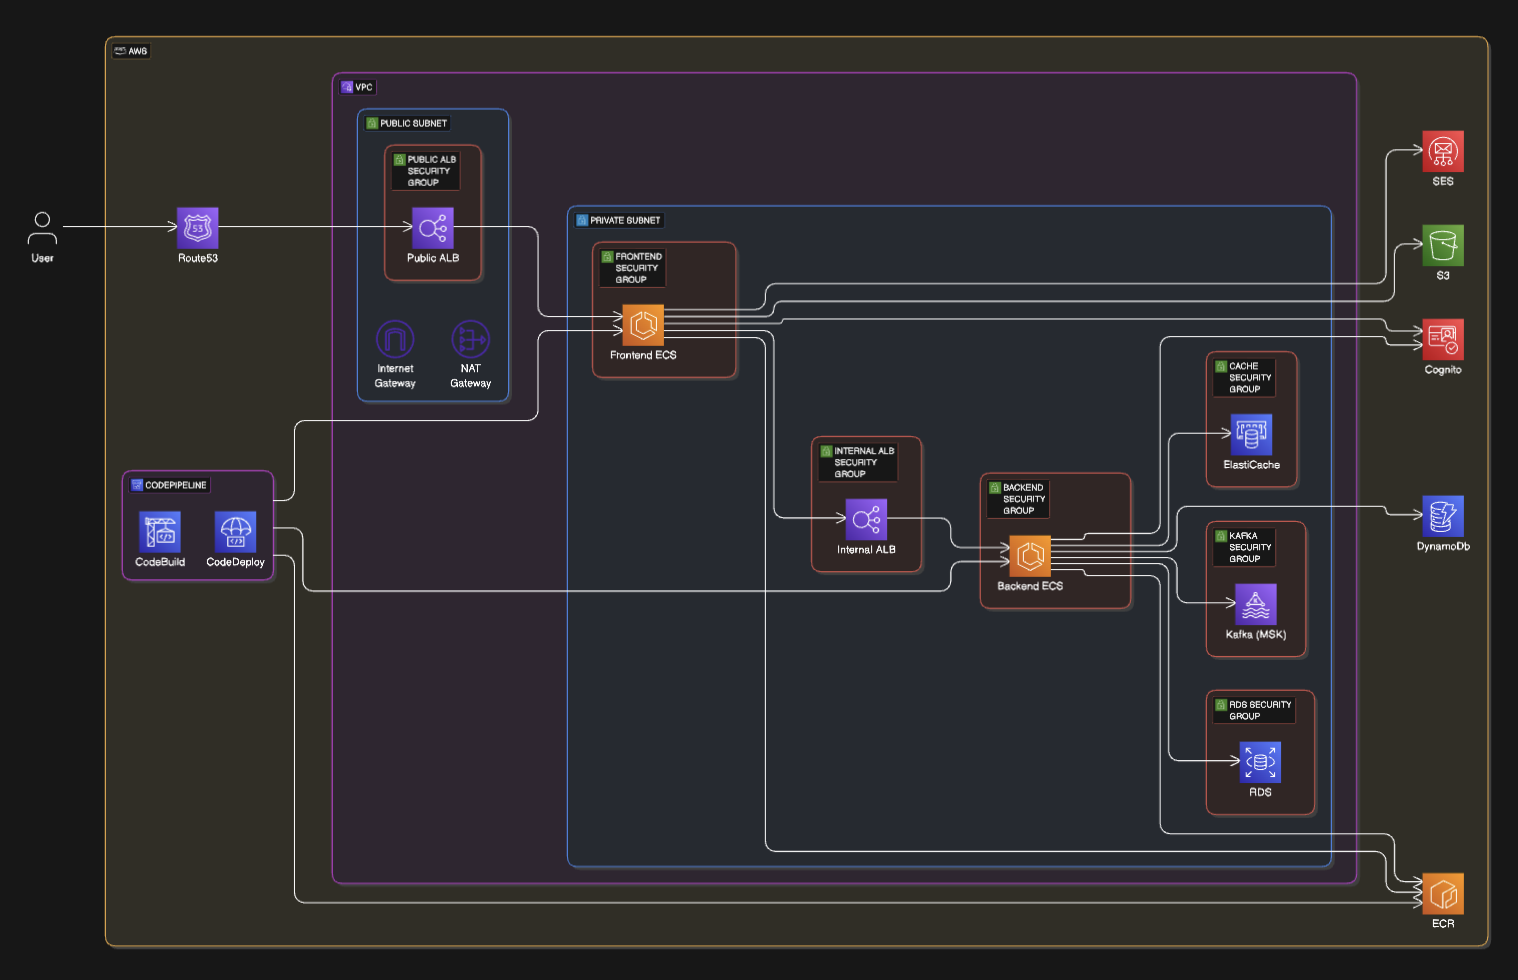
\includegraphics[width=\textwidth]{FinalArchitectureDiagram.png}

The diagram above shows the AWS architecture, it includes three main sections, the services inside the Virtual Private Cloud (VPC), the Global AWS Services and the services in Codepipeline. While all of these services interact, there separation is important, and it is based on how AWS setup their services. The services that were used were primarily chosen based on the initial technology stack but they also have their own benefits which will be discussed.

\subsubsection{VPC Services}

The services inside the VPC are deployed across multiple availabilty zones and if needed they can be deployed across different AWS regions for enhanced global coverage. The diagram shows the interactions between each services. 

\paragraph{Subnets}

Subnets are range of IP addresses, the difference between the public and private subnets is that the public ones have direct access to an internet gateway and public traffic can be made accessible to them, whereas the private subnets do not allow any public ingress and they can egress using the NAT Gateway.

\paragraph{Security Groups}
A security group controls the traffic that is allowed to reach and leave the resources that it is associated with \cite{aws_sg}. They surround all of the services and only allow the correct traffic, for example the backend ALB will only accept traffic from the frontend security group. This adds an extra layer of security to the deployment. 

\paragraph{Load Balancers}

Application Load Balancers (ALB's) are used to automatically distribute incoming application traffic across multiple targets, such as the ECS services above. This project utilizes two different Load balancers, there is a public ALB which is accessible from the internet and it routes user traffic to the frontend containers. Then there is an internal ALB which routes the frontend's requests to the backend containers, this architecture was created so that the two services can scale independently. The ALB's have health checks for their downstream services so they will only send traffic to healthy tasks and will force redeployment of unhealthy tasks.

\paragraph{Elastic Container Service (ECS)}
The ECS services contain docker containers for a specific task, such as the frontend and backend of this project. They are serverless as they are being run with AWS Fargate, which means that the underlying servers are managed by AWS.

\paragraph{Elasticache}
Amazon ElastiCache is a serverless, fully managed cache delivering real-time, cost-optimized performance for data-driven applications \cite{aws_cache}, it is being used to host a cluster of Redis caches for the backend. ElastiCache Serverless means zero infrastructure management, zero downtime maintenance, and instant scaling to match any application demand \cite{aws_cache}. 

\paragraph{Managed Streaming for Apache Kafka (MSK)}
Amazon MSK is a streaming data service that manages Apache Kafka infrastructure and operations, making it easier for developers and DevOps managers to run Apache Kafka applications \cite{aws_msk}. Amazon MSK operates, maintains, and scales Apache Kafka clusters, provides enterprise-grade security features out of the box, and has built-in AWS integrations \cite{aws_msk}. This service allows for easy and secure Kafka clusters to be used with the backends service as discussed above which is why it was chosen over other solutions.

\paragraph{Relational Database Service (RDS}
Amazon Relational Database Service (Amazon RDS) is an easy-to-manage relational database service \cite{aws_rds}. Amazon RDS automates undifferentiated database management tasks, such as provisioning, configuring, backing up, and patching \cite{aws_rds}. This was decided as the best way to host the Postgres Database on AWS.


\subsubsection{Global Services}

\paragraph{Elastic Container Registry (ECR)}
ECR is a fully managed container registry which is storing the frontend and backend docker images after they have been built in CodeBuild.

\paragraph{Simple Email Service (SES)}
SES is an AWS service that can be used for sending emails to clients, and internally, this project uses it to send the get in contact emails from users, it has a Javascript integration so it was easy to add to the frontend. 


\paragraph{S3}
Amazon Simple Storage Service (Amazon S3) is an object storage service offering industry-leading scalability, data availability, security, and performance \cite{aws_s3}. It is being used in this project to store and host users item's images so that they can be used within the application. You can store virtually any amount of data with S3 all the way to exabytes with unmatched performance \cite{aws_s3} which means that the developers do not have to worry about the amount of images the users are uploading.

\paragraph{Route53}
Route53 is AWS's Domain Name System (DNS), while any DNS could have been used as they are all very similar, Route53 was chosen due to its integration with other AWS services and how easy it was to point DNS records at Load balancers inside AWS which made Route53 ideal for this project.

\paragraph{DynamoDB}
Above in technologies section under  \nameref{subsubsec:database:technology:dynamo}, the reasons why DynamoDb was chosen were outlined and some more of the benefits are that DynamoDB scales to zero, has no cold starts, no version upgrades, no maintenance windows, no patching, and no downtime maintenance. DynamoDB offers a broad set of security controls and compliance standards \cite{aws_dynamodb}.

\paragraph{Cognito}
Cognito is a developer-centric, cost-effective service that provides secure, tenant-based identity stores and federation options that can scale to millions of users \cite{aws_cognito}, in this project it is used for authentication, to control user accounts as well as JWT authorization and more.

\subsubsection{CodePipeline}

AWS CodePipeline is a continuous integration and continuous delivery (CI/CD) service for fast and reliable application and infrastructure updates \cite{aws_codepipeline}. It has multiple integrations with source code providers which means that the pipelines can be ran on code updates. This project uses it to control the majority of the CI/CD and it has been configured to use Codebuild and CodeDeploy to manage building new releases and deploy them, below is the pipeline.

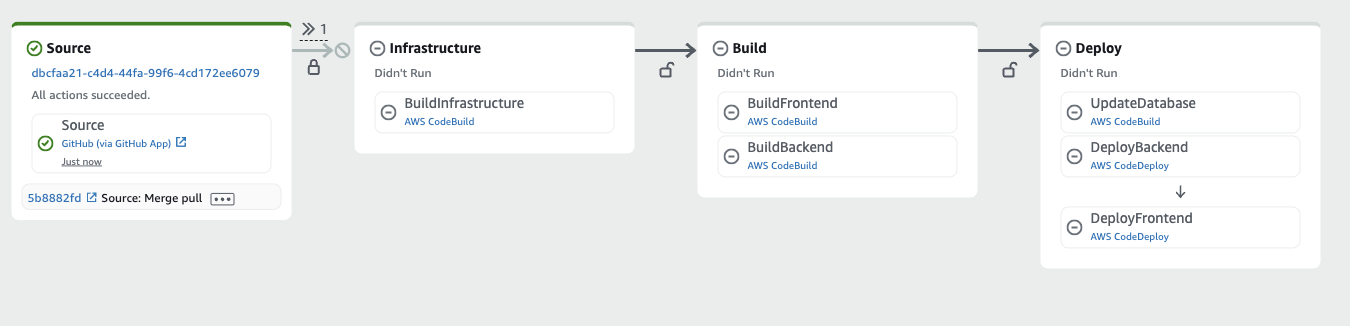
\includegraphics[width=\textwidth]{images/CodePipeline.png}

This image shows the steps in the pipeline and how it is configured, first the source code is retrieved, then in the Infrastructure step a Codebuild project is ran which updates the deployed infrastructure. Then the frontend and backend are built and pushed to ECR, and finally the database is updated and the services are updated using a blue green canary deployment. If any of these stages fail the next steps will not run which means prevents faulty updates being deployed.


\subsection{Docker Architecture}

When deploying this using the Docker stack on a server there are differences to how it is deployed on AWS, below is a diagram on how the containers are ran.

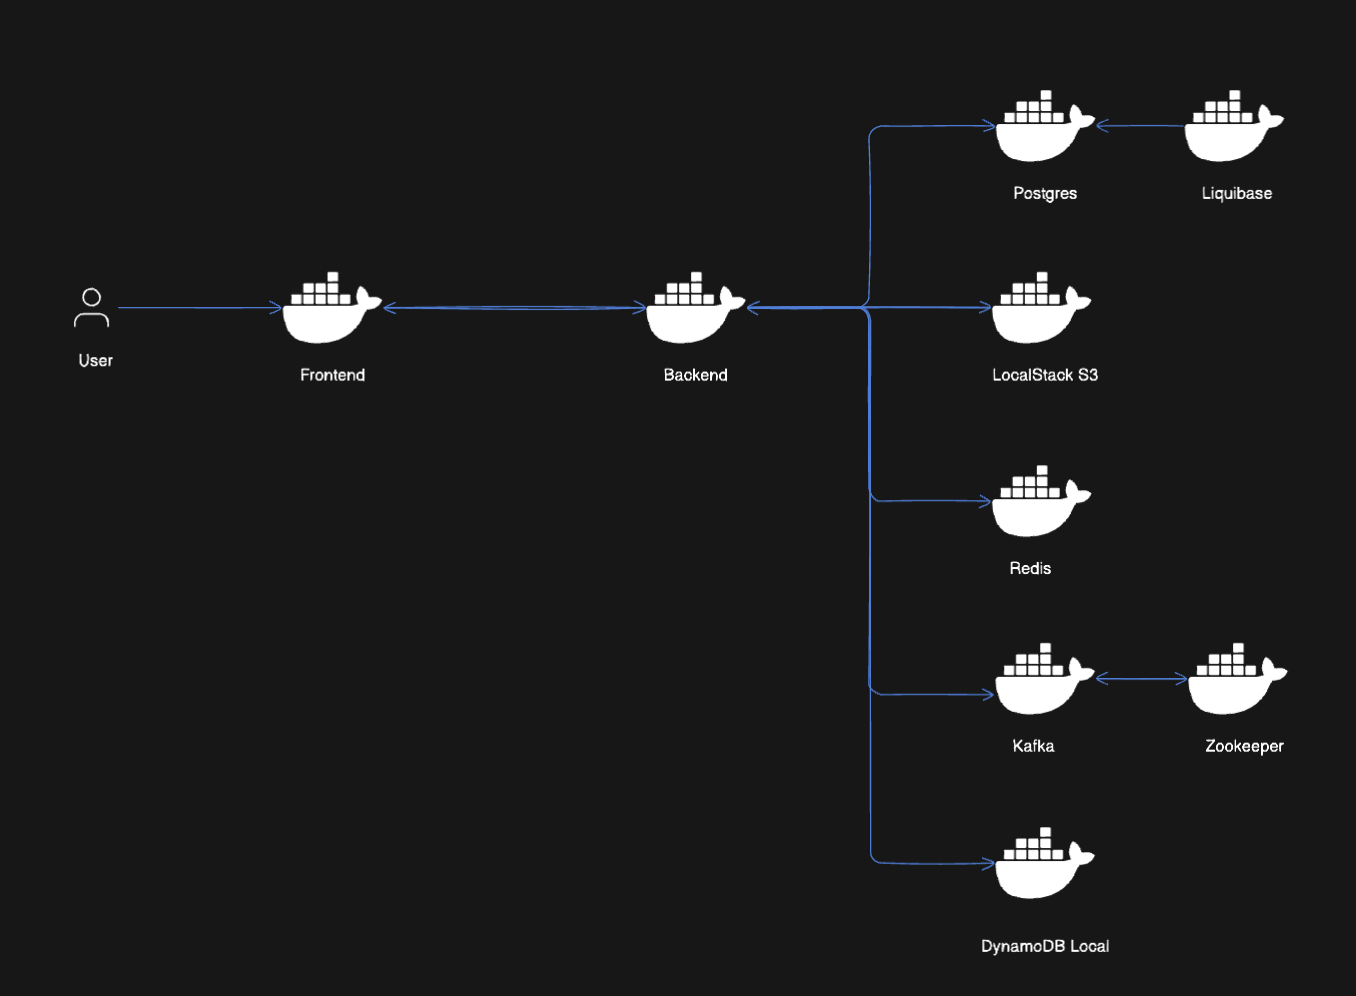
\includegraphics[width=\textwidth]{images/DockerStackArchitecture.png}

The main difference is the simplicity of the architecture and how there is less restrictions around how the services communicate with each other, there is less architectural security like there is with AWS security groups. Secondly, it is missing these: load balancing, CI/CD, Cognito and SES, while it is possible to add these to the project later on there is no local version or alternative of Cognito and it is essential to this application so this must be hosted on AWS no matter how the application is deployed. 


\section{Database Design}

\subsection{Relational Database}
\includegraphics[width=\textwidth]{DatabaseUML.png}

The initial database model was designed based on the required information about users, and on research of online shops and what information they show, then as the application progressed and evolved so did the data model. Above is the Unified Modelling Language (UML) diagram of the final model and it shows how the tables are linked together. Using UML throughout development helped identify potential design issues early in on, such as unnecessary dependencies or missing attributes.

Every table contains a last updated at and created at value which are used for auditing purposes, these values update based on triggers so that they are always updated. Finally to confirm the database designs and query functionality there is a separate test schema that contains procedures for testing all of the functions.

\subsection{NoSQL Database}

The DynamoDB NoSQL database has a minimal schema that is flexible, it includes table keys and indexes. For example below is the schema of the development tables, in the dev chats table there are the hash and range keys which are the conversationId and the createdAt and then there are two global secondary indexes (GSI's) which are the chatId and the userId. The keys allow the application to retrieve all chats where the conversationId is know and or all chats in a specific time period and the indexes allow the application to query the data on these different columns (This requires extra read and write capacity).

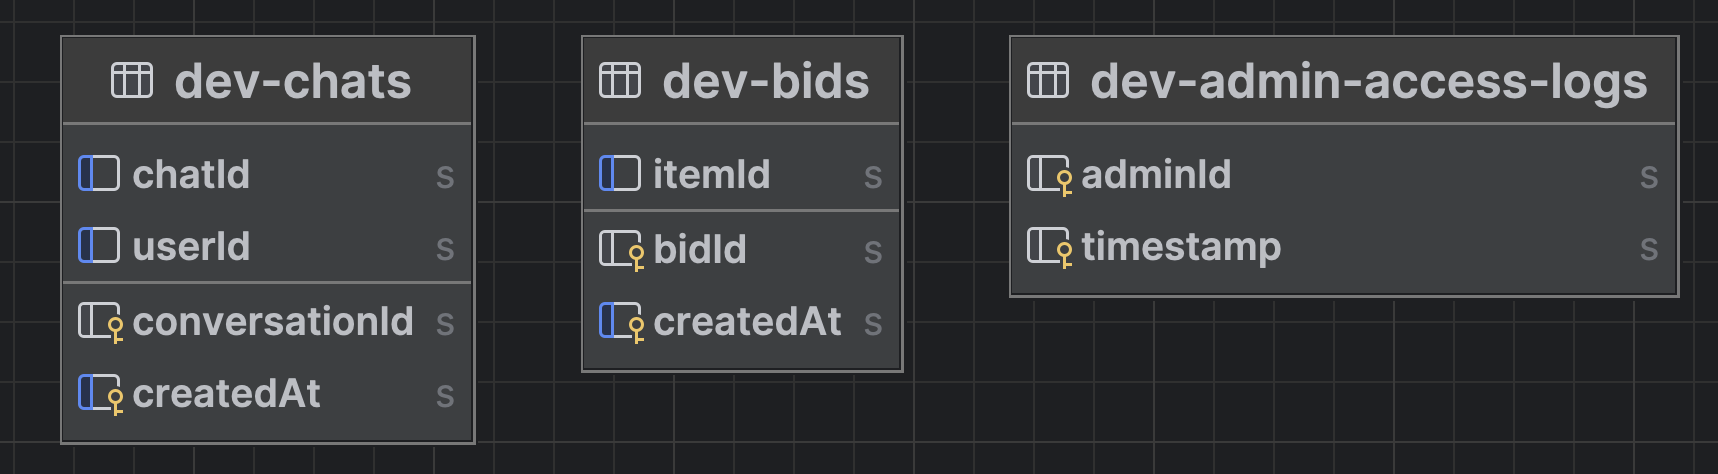
\includegraphics[width=\textwidth]{NoSQLDiagram.png}

\section{Features}

This section contains some of the most important features that were completed.

\subsection{AI Chatbot}

\begin{codeblock}[H]
    \begin{minted}[
        gobble=0 
    ]{javascript}
        const optimisticChat: Chat = {
        __typename: "Chat",
        chatId: optimisticChatId,
        conversationId: currentConversationId,
        message: newMessage,
        sender: "User",
        createdAt: new Date().toISOString(),
      };

      // Optimistically update the conversation state
      setConversation((prev) => [...prev, optimisticChat]);

      createChatMutation({
        variables: {
          conversationId: currentConversationId,
          message: newMessage,
        },
        onCompleted: (data) => {
          if (data?.createChat) {
            const { response } = data.createChat;

            // Remove optimistic chat and replace with actual chat and response
            setConversation((prev) => [
              ...prev,
              ...[response].filter(
                (msg): msg is Chat => msg !== null && msg !== undefined,
              ),
            ]);
          }
        },
        onError: (error) => {
          console.error("Error sending message:", error);
          // Remove optimistic chat on error
          setConversation((prev) =>
            prev.filter((msg) => msg.chatId !== optimisticChatId),
          );
        },
      });
\end{minted}
    \caption{JavaScript code for optimistic UI update in chat.}
    \label{code:optimistic-chat}
\end{codeblock}

The AI Chat bot allows users to ask for help and the response is generated by a large language model (LLM), this is important as it allows the users get the help they need while also allowing the team behind the project to not be swamped by responding to these messages. 

The chatbot works using Graphql queries and mutations but there are also some interesting parts of code that enhance the user experience. Firstly, there is optimistic updating of the chats, this means that the second a user has sent a message, their message is updated on the UI even before the mutation has been fired. The code for this is above \ref{code:optimistic-chat}:

\begin{codeblock}[H]
    \begin{minted}[
        gobble=0 
    ]{java}
        OpenAIClient client = OpenAIOkHttpClient.builder()
              .apiKey(openAiApiKey)
              .project(openAiProject)
              .organization(openAiOrganization)
              .build();

      String prompt =
              "You are a friendly, helpful assistant for an "
                      + "online shopping platform called SubShop. "
                      + "Your name is SmartShop Assistant. "
                      + "Respond in a warm, conversational tone while being concise and accurate. "
                      + "Address the user directly and personalize your responses. "
                      + "If you cannot answer based on your knowledge, politely "
                      + "explain you're unable to help "
                      + "and suggest contacting customer service. "
                      + "End your response with a follow-up question or "
                      + "offer of additional help when appropriate. "
                      + "User's Question: "
                      + message;

      ResponseCreateParams params = ResponseCreateParams.builder().input(prompt).model(ChatModel.GPT_4O_MINI).build();

      Response response = client.responses().create(params);
\end{minted}
    \caption{Java code for creating chats with OpenAi.}
    \label{code:create-chat}
\end{codeblock}

Secondly, there is the way that the chat is created by OpenAI and the prompt that OpenAI receives, the code is above \ref{code:create-chat}. This code shows how interactions with third party SDK's but also how the LLM is prepared to answer the questions it receives. There is a better solution to this problem that would involve hosting an independent LLM that uses Retrieval-Augmented Generation (RAG) to get application specific information so that the answers created are much better.


\subsection{Searching}

\begin{codeblock}[H]
    \begin{minted}[
        gobble=0 
    ]{SQL}
 IF NOT EXISTS (
        SELECT 1
        FROM pg_attribute
        WHERE attrelid = 'items'::regclass
          AND attname = order_by
          AND attnum > 0
          AND NOT attisdropped
    ) THEN
        RAISE EXCEPTION 'Invalid column name for ordering: %', order_by;
    END IF;

    RETURN QUERY EXECUTE format(
        'SELECT
            i.item_id, 
            i.name, 
            i.description,
            i.is_active,
            i.ending_time,
            i.price,
            i.stock,
            i.category,
            i.images,
            i.seller_id,
            i.final_price
        FROM items i
        WHERE similarity(i.name, $1) > 0.3
        AND is_active = true
        ORDER BY %I %s
        LIMIT $2 OFFSET $3', 
        order_by,
        order_direction
    )
     USING search_text, page_size, page * page_size;
END;
$$ LANGUAGE plpgsql;
\end{minted}
    \caption{SQL for searching for items.}
    \label{code:search-for-items}
\end{codeblock}

This part of the code shows the database searching for items method, it uses the pg\_trgm extension to get a similarity score of how close the search text is to the names of the items in the database. Currently the similarity score is set to be over 0.3 to try and match lots of items and the items are ordered on how closely matched they are which means that users will get the best results first. The inner function returns a query so that the correct table data can be returned into the returns table query. A plpgsql function is being used so that a more of the logic can be added into the schema rather than duplicating logic in the layers above. 

As mentioned earlier in the \nameref{subsection:sqlinjection} sub section it was discussed why this function is good from a security standpoint but there are also risks. The order by column name is as input from the client, while there is a check for verifying it is a valid table there are still security issues with this. 

The benefits aside from searching, the order by feature and pagination are important user features as they can help a user interact with the searched data as there will be less information on the UI and they can order it whatever way they want. Secondly the pagination helps the server load as not all of the information is returned every query.

\subsection{User payments}
User to User payments was enabled thanks to Stripe Connect, but the implementation of it is an essential part of this project so it should be highlighted. First, the payment flow must be decided, for security reasons the payment information should all be handled by Stripe and when a user places a bid, the payment needs to be authorized upfront to guarantee the availability of funds and allow the user to resolve any potential card issues (like 3D Secure authentication) immediately. This is achieved using a Stripe SetupIntent, the SetupIntent is created on the Frontends server using the code below \ref{code:createSetupIntent}: 

\begin{codeblock}[H]
    \begin{minted}[
        gobble=0 
    ]{javascript}
    const setupIntent = await stripe.setupIntents.create({
      customer: customerId,
      payment_method_types: ["card"],
      usage: "on_session",
      metadata: {
        item_id: itemId,
        bid_amount_gbp: (amount / 100).toFixed(2),
        reason: `Bid authorization for item ${itemId}`,
      },
      description: `Authorize card for bid on item ${itemId}`,
    });

    return NextResponse.json({
      success: true,
      clientSecret: setupIntent.client_secret,
    });
\end{minted}
    \caption{Frontend API for setup intents.}
    \label{code:createSetupIntent}
\end{codeblock}

Once the SetupIntent is created the client secret is returned so that it can be linked in the Stripe elements for confirmation of the SetupIntent and it is confirmed by using the code below \ref{code:confirmSetupIntent}. If successful, Stripe securely saves the payment method details associated with the user's Stripe Customer ID and links it to the SetupIntent. It is linked to the created Setup Intent by the Stripe elements. The SetupIntent is returned so that the paymentMethodId \mint{javascript}|const paymentMethodId = setupIntent.payment_method;| can be sent to the backend for finalisation.

\begin{codeblock}[H]
    \begin{minted}[
        gobble=0 
    ]{javascript}
    const { error, setupIntent } = await stripe.confirmSetup({
      elements,
      confirmParams: {
        return_url: `${window.location.origin}/shop/item/${itemId}`,
      },
      redirect: "if_required",
    });
\end{minted}
    \caption{Frontend confirmation of setup intents.}
    \label{code:confirmSetupIntent}
\end{codeblock}

Now that the payment has been authorized, once the auction has completed the winning payment needs to be confirmed and processed. This process is being completed in the backends closed auction consumer, it reads the closed auctions, completes the payments and updates the database. It gets both the buyer and sellers stripe information from the database and then uses the PaymentMethodId that was generated in the previous step \label{code:confirmSetupIntent}. The transfer information is set so that stripe confirms the payment without immediate approval as the user is off session and has already confirmed it. Below is the code described \label{code:createPaymentIntent}

\begin{codeblock}[H]
    \begin{minted}[
        gobble=0 
    ]{java}
    PaymentIntentCreateParams.Builder paramsBuilder = PaymentIntentCreateParams.builder()
              .setAmount(amountInPence)
              .setCurrency("GBP")
              .setCustomer(customerId)
              .setPaymentMethod(finalBid.getPaymentMethod())
              .setConfirm(true)
              .setOffSession(true)
              .setCaptureMethod(PaymentIntentCreateParams.CaptureMethod.AUTOMATIC)
              .setTransferData(
                      PaymentIntentCreateParams.TransferData.builder()
                              .setDestination(sellerId)
                              .build()
              )
              .putMetadata("item_id", item.getId().toString())
              .putMetadata("bidder_user_id", finalBid.getUserId().toString())
              .putMetadata("seller_user_id", item.getSeller().toString());

      PaymentIntent.create(paramsBuilder.build());
\end{minted}
    \caption{Backend creation of payment intent.}
    \label{code:createPaymentIntent}
\end{codeblock}


\subsection{Redis Leader Election Service }

This code implements a leader election mechanism using Redis as a distributed lock provider. The goal is to ensure that among potentially multiple instances of the application running concurrently, only one instance holds the "leadership" status at any given time. The leader instance is responsible for getting items from completed auctions and publishing them to a Kafka topic.

Firstly each instance checks if they are the leader and if they are then they will try and extend their leadership. Otherwise they will try and become the leader and if there is an existing leader they wait until the scheduled heartbeat, which is a function that runs every 30 seconds, and then try again. If there are any errors during the leader election the instance checks if they are the leader and if they are they will remove themselves as leader so that the other instances can take over while the error is being investigated. The code for this is below \label{code:leadership service}.

\begin{codeblock}[H]
    \begin{minted}[
        gobble=0 
    ]{java}
    private final AtomicBoolean isLeader = new AtomicBoolean(false);

      @Scheduled(fixedRate = LEADER_EXPIRY_SECONDS * 1000 / 3)
      public void leadershipHeartbeat() {
        attemptToAcquireOrRefreshLeadership();
      }
  
    private void attemptToAcquireOrRefreshLeadership() {
    try (Jedis jedis = jedisPool.getResource()) {
      LocalDateTime now = LocalDateTime.now(ZoneOffset.UTC);
      String timestamp = now.format(FORMATTER);
      String hostInfo = getHostInfo();

      AppLogger.info("Attempting to acquire leadership for host: " + hostInfo);
      if (isLeader()) {
        // Already the leader, try to extend the lease
        String currentLeader = jedis.get(LEADER_KEY);
        if (instanceId.equals(currentLeader)) {
          // Still the leader, reset expiry
          jedis.expire(LEADER_KEY, LEADER_EXPIRY_SECONDS);
          AppLogger.info("Instance {} leadership renewed at {}", instanceId, timestamp);
        } else {
          // Lost leadership
          isLeader.set(false);
          AppLogger.info("Instance {} lost leadership at {}", instanceId, timestamp);
        }
      } else {
        // Try to become the leader using SET NX EX (only set if not exists with expiry)
        String result = jedis.set(LEADER_KEY, instanceId,
                SetParams.setParams().nx().ex(LEADER_EXPIRY_SECONDS));

        if ("OK".equals(result)) {
          isLeader.set(true);
          AppLogger.info("Instance {} acquired leadership at {} on {}",
                  instanceId, timestamp, hostInfo);
        }
      }
    } catch (Exception e) {
      AppLogger.error("Error in leader election: {} at {}",
              e.getMessage(), LocalDateTime.now(ZoneOffset.UTC).format(FORMATTER));

      // On error, assume not the leader for safety
      if (isLeader()) {
        isLeader.set(false);
        AppLogger.warn("Instance {} relinquishing leadership due to error", instanceId);
      }
    }
  }
\end{minted}
\caption{Backend redis leadership service.}
\label{code:leadership service}
\end{codeblock}

\subsection{Infrastructure shared between local and remote states}

The final piece of code being discussed is how infrastructure that is to be applied to AWS can also be deployed to Docker containers and the best ways for this. Firstly, code duplication is unwanted, it would be easiest to create local and remote version of the code and update both each time an update was needed. 

This problem was solved by creating a shared and a local directory of terraform code alongside the remote directory. This means that the remote configuration can stay the same and the local provider can be altered to use the local endpoints as seen in the code block below \label{code:terraformProvider}.

\begin{codeblock}[H]
    \begin{minted}[
        gobble=0 
    ]{terraform}
terraform {
  required_version = ">= 1.9"
  required_providers {
    aws = {
      source  = "hashicorp/aws"
      version = ">= 5.60.0"
    }
  }
}

provider "aws" {
  region = "eu-west-2"

  access_key                  = "test"
  secret_key                  = "test"
  skip_credentials_validation = true
  skip_metadata_api_check     = true
  skip_requesting_account_id  = true

  s3_use_path_style = true


  dynamic "endpoints" {
    for_each = toset(["dynamodb", "s3"])
    content {
      dynamodb = "http://localhost:8000"
      s3       = "http://localhost:4566"
    }
  }

  default_tags {
    tags = {
      Environment = "local"
      Project     = "SubShop"
    }
  }
}
\end{minted}
\caption{Local terraform provider.}
\label{code:terraformProvider}
\end{codeblock}

Now that both the local and remote providers are setup, the same IaC can be added to the shared directory and used like any other module, this is shown below \label{code:terraformModules} where in the remote main.tf there is a s3 module and a shared\_s3 module. This approach creates one source of truth for the shared infrastructure which enhances the development experience. 

\begin{codeblock}[H]
    \begin{minted}[
        gobble=0 
    ]{terraform}
module "s3" {
  source = "./modules/s3"

  environment               = var.environment
  codepipeline_iam_role_arn = module.iam.codepipeline_role_arn
  codebuild_iam_role_arn    = module.iam.codebuild_role_arn
  codedeploy_iam_role_arn   = module.iam.codedeploy_service_role_arn
}

module "shared_s3" {
  source = "../shared/s3"

  environment     = var.environment
  allowed_origins = [var.domain]
}
\end{minted}
\caption{Remote Terraform shared and private modules..}
\label{code:terraformModules}
\end{codeblock}

\chapter{Installation and User manual}
\label{chapter:installation}

This chapter will cover the high level steps to install the application and a user manual so that potential users can look at this to run and use the application. There is a more in-depth installation and running instructions inside the source code if there are any issues.

\section{Installation}
There are some prerequisites to running the application on both Docker and AWS, first you need to setup Stripe \url{https://stripe.com/gb} so that you can accept payments from subscriptions as well as enable payments between users, and for this you need to sign up for Stripe connect. Then you need to create a subscription and get the priceId of it so that it can be used inside the application. 

Whether deploying with either method, Cognito must be setup, and for this you will need to create an AWS account and setup the correct IAM roles so that you can get AWS credentials with access to the resources needed to create the infrastructure. To setup Cognito, open an command line, ensure terraform is installed, setup your AWS access keys using the AWS CLi. Then navigate to the remote infrastructure directory and run: \mint{shell}|terraform apply -target=module.cognito| This will setup Cognito, then you can use the AWS console to get the required environment variables for it.

For more detailed instructions follow the README's inside the source code.

\subsection{Docker}
To run the application using Docker, you first need to ensure Docker is installed on the platform that you are building the application on. If it is then you can proceed to setting it up. Open a Command line and navigate to the docker directory in the product, then setup the environment variables by following the README and finally run the containers using: \mint{shell}|docker compose -f docker-compose-local.yml up -d| Once this is done then to apply the local infrastructure go to the local infrastructure directory and run  \mint{shell}| terraform apply | like how it was done for setting up Cognito. After all of that the application will be ready.

\subsection{AWS}

When deploying to AWS the steps are slightly different, it is recommended that you initially build the Frontend and backend Docker images, to do so go to their respective directories and follow the instructions. 

Next you want to build the infrastructure using terraform, to do so navigate to the remote terraform directory, setup the enviroment variables using the example files and the instrustions in the README, then setup the terraform backend to use GitLab terraform states as discussed above or use a different terraform backend, then run: \mint{shell}| terraform apply |
This will start to create the infrastructure, but there are some manual steps that need completing these are also contained in the main infrastructure README, first you need to complete the codeconnections authentication so that the CI/CD pipelines will be able to run correctly, then you need to enable production mode for SES. These steps both have guides from amazon for doing this. Finally you need to get the name servers of the Route53 hosted zone and set your domain to point at them. 

Another tip would be to push the Docker images to ECR with the latest tag before all of the deployment is completed, this will ensure the ECS services are failing to deploy while waiting for the CI/CD pipelines to finish as there will be an existing image in the repository. The steps for this will be inside ECR under view push commands. 

After the infrastructure is built and the CI/CD pipeline is completed the application will be ready to receive traffic.

\section{User manual}
\subsection{General Use}
Once the code is up and running these steps will help you navigate the application. The first step is going to the application either by using the domain you configured or the address of it. Then you want to sign up as a new user using your details:

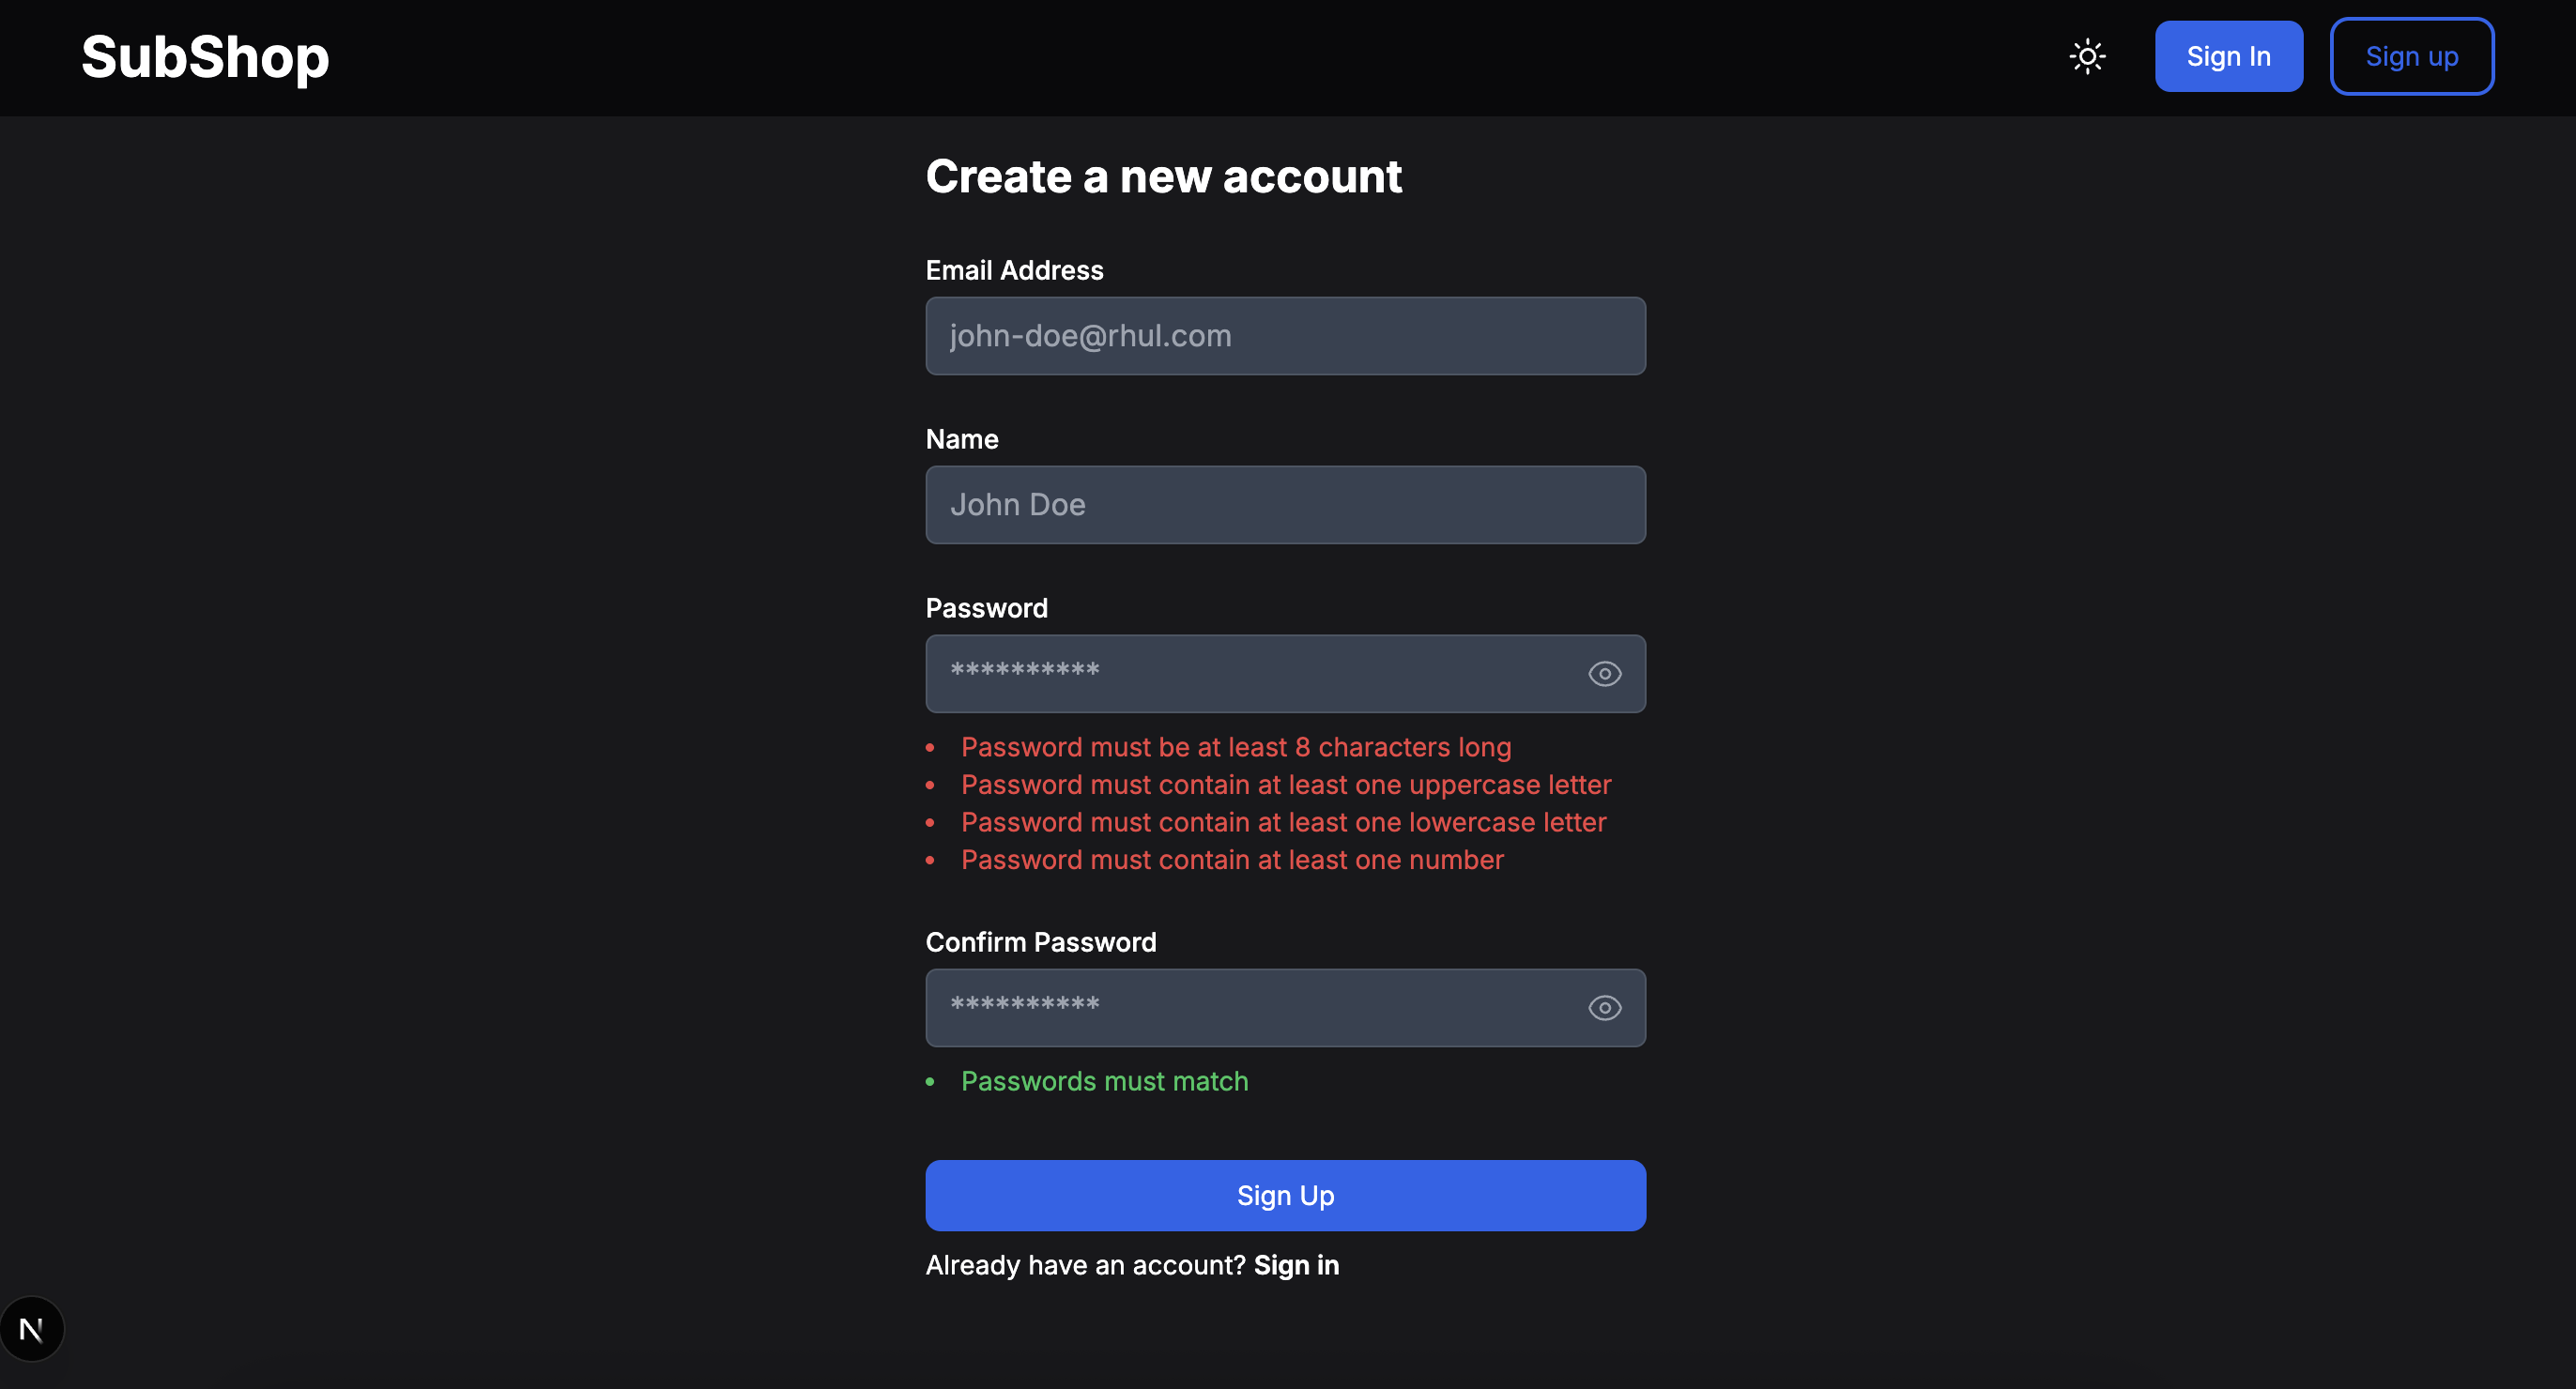
\includegraphics[width=\textwidth]{CreateAccount.png}

Once you have created an account you will be redirected to the accounts page, once here you will need to follow the highlighted steps to complete your account setup. After that you are free to use the application or register as a seller. There are also buttons here that allow you to delete your account or report an issue, the delete account button will remove your account and revoke access, and the report button will create a ticket in the configured Jira account with all the details from the user.

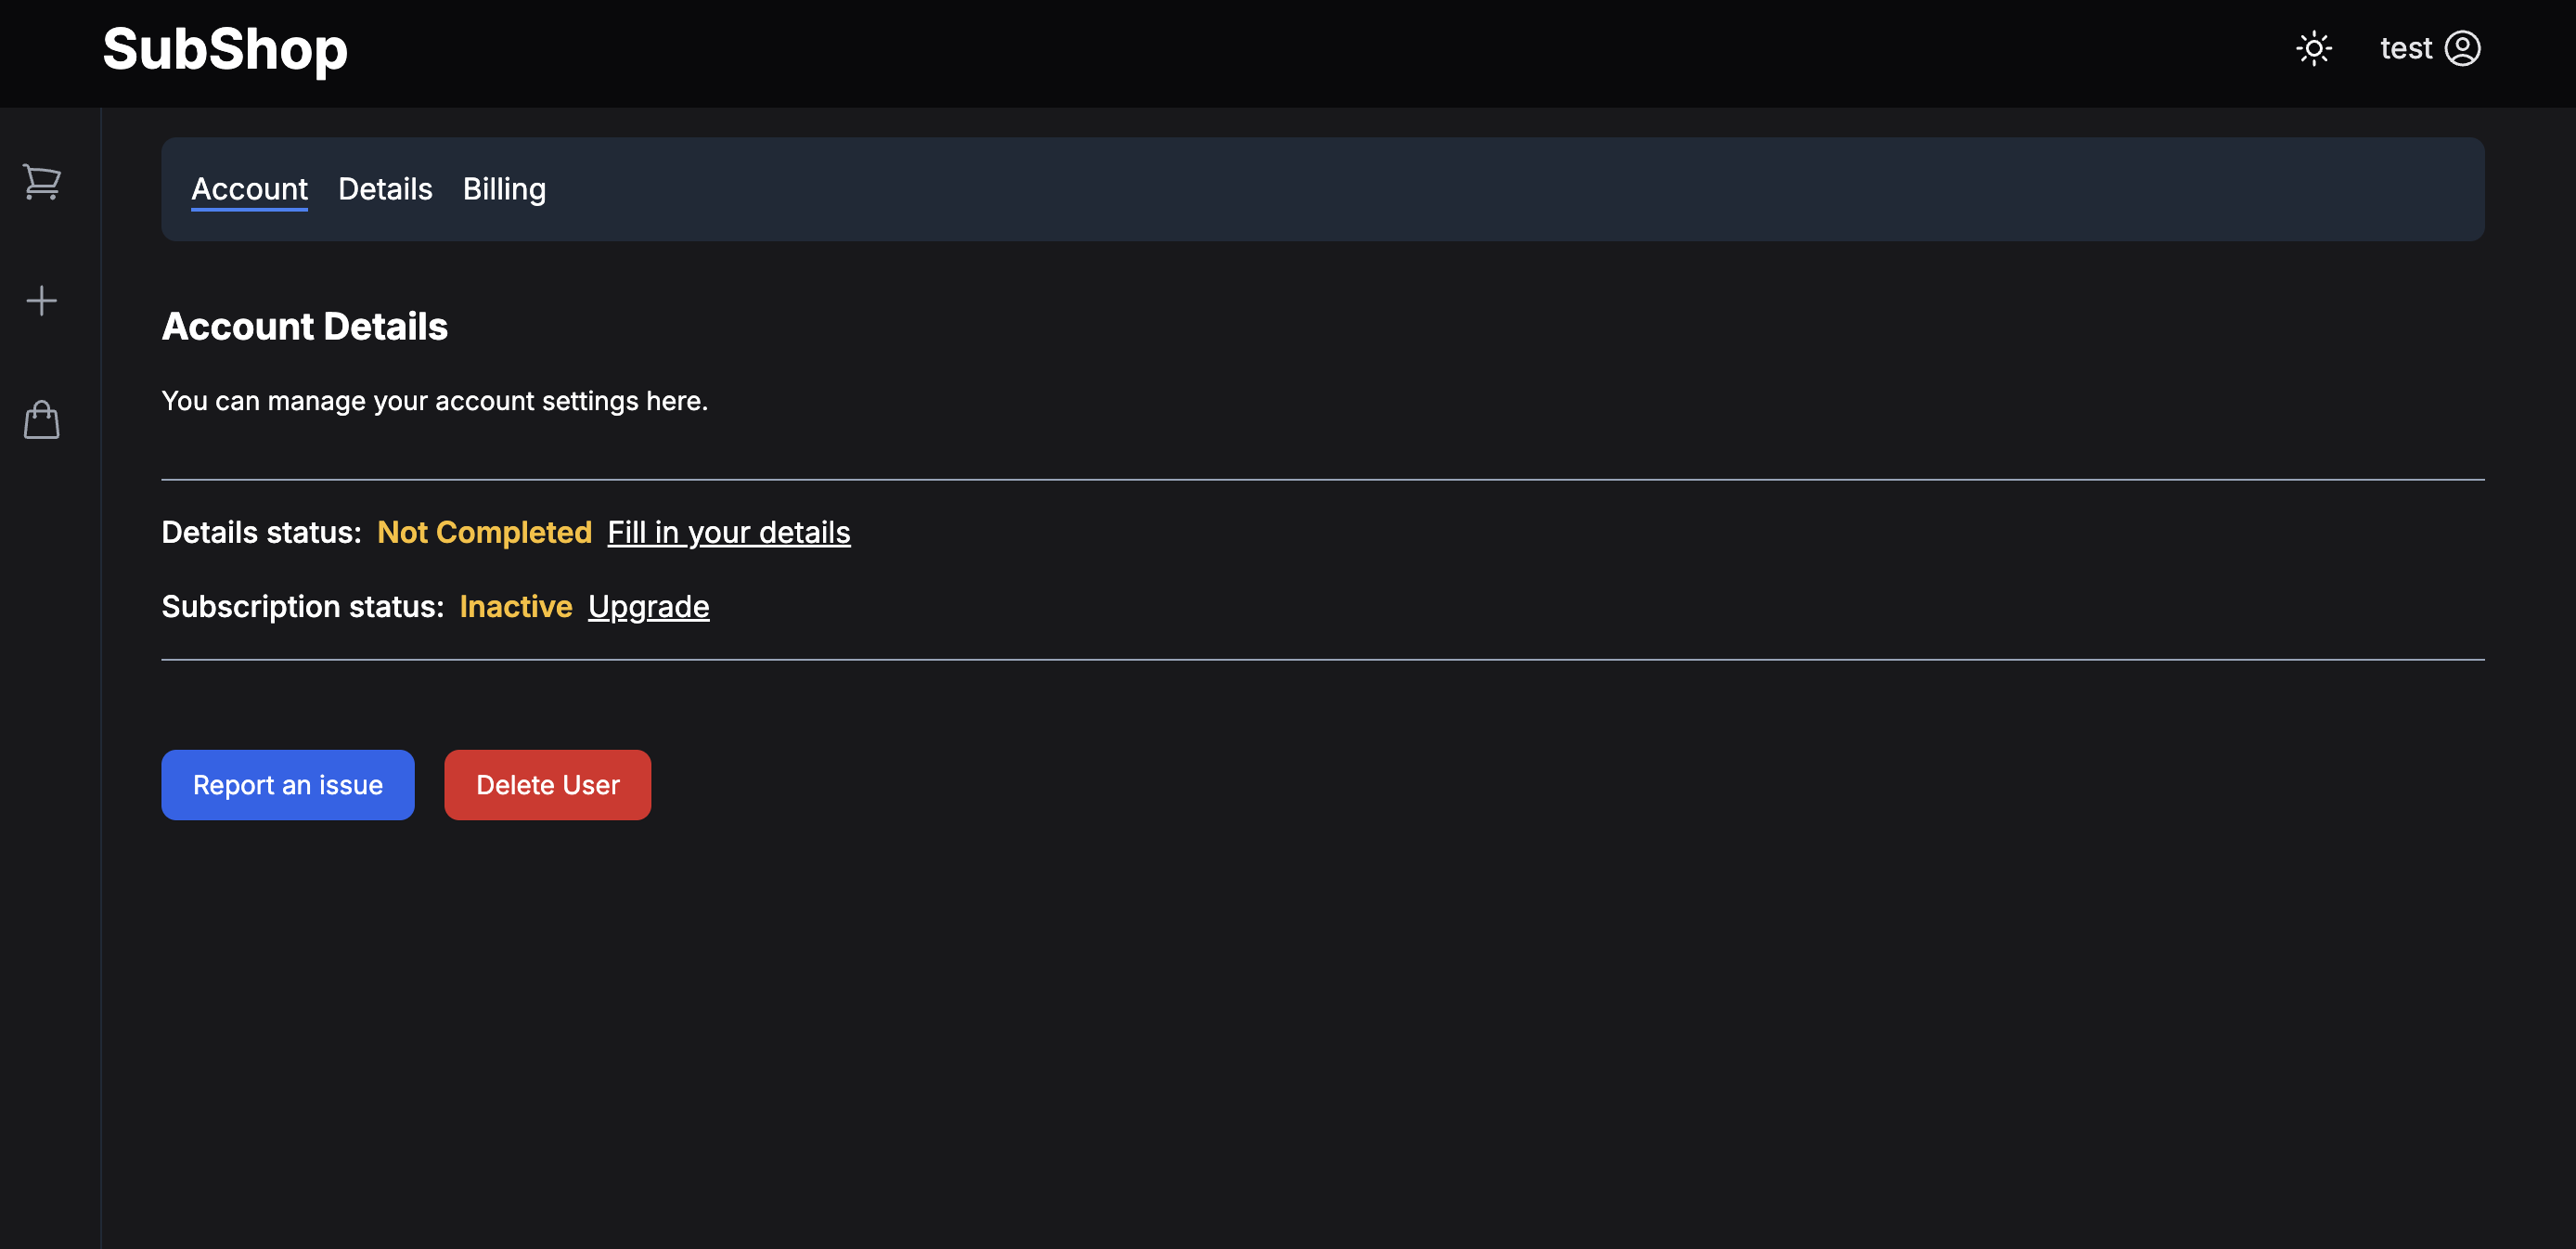
\includegraphics[width=\textwidth]{ManageAccount.png}

After you have set up an account you can go create new items, or browse other peoples items in the shop. As seen below there are some items already in the shop and there is a helpful chat window for you to ask questions with. The shop page contains all of the active auctions on the platform as well as give you a way to search for specific items you want.

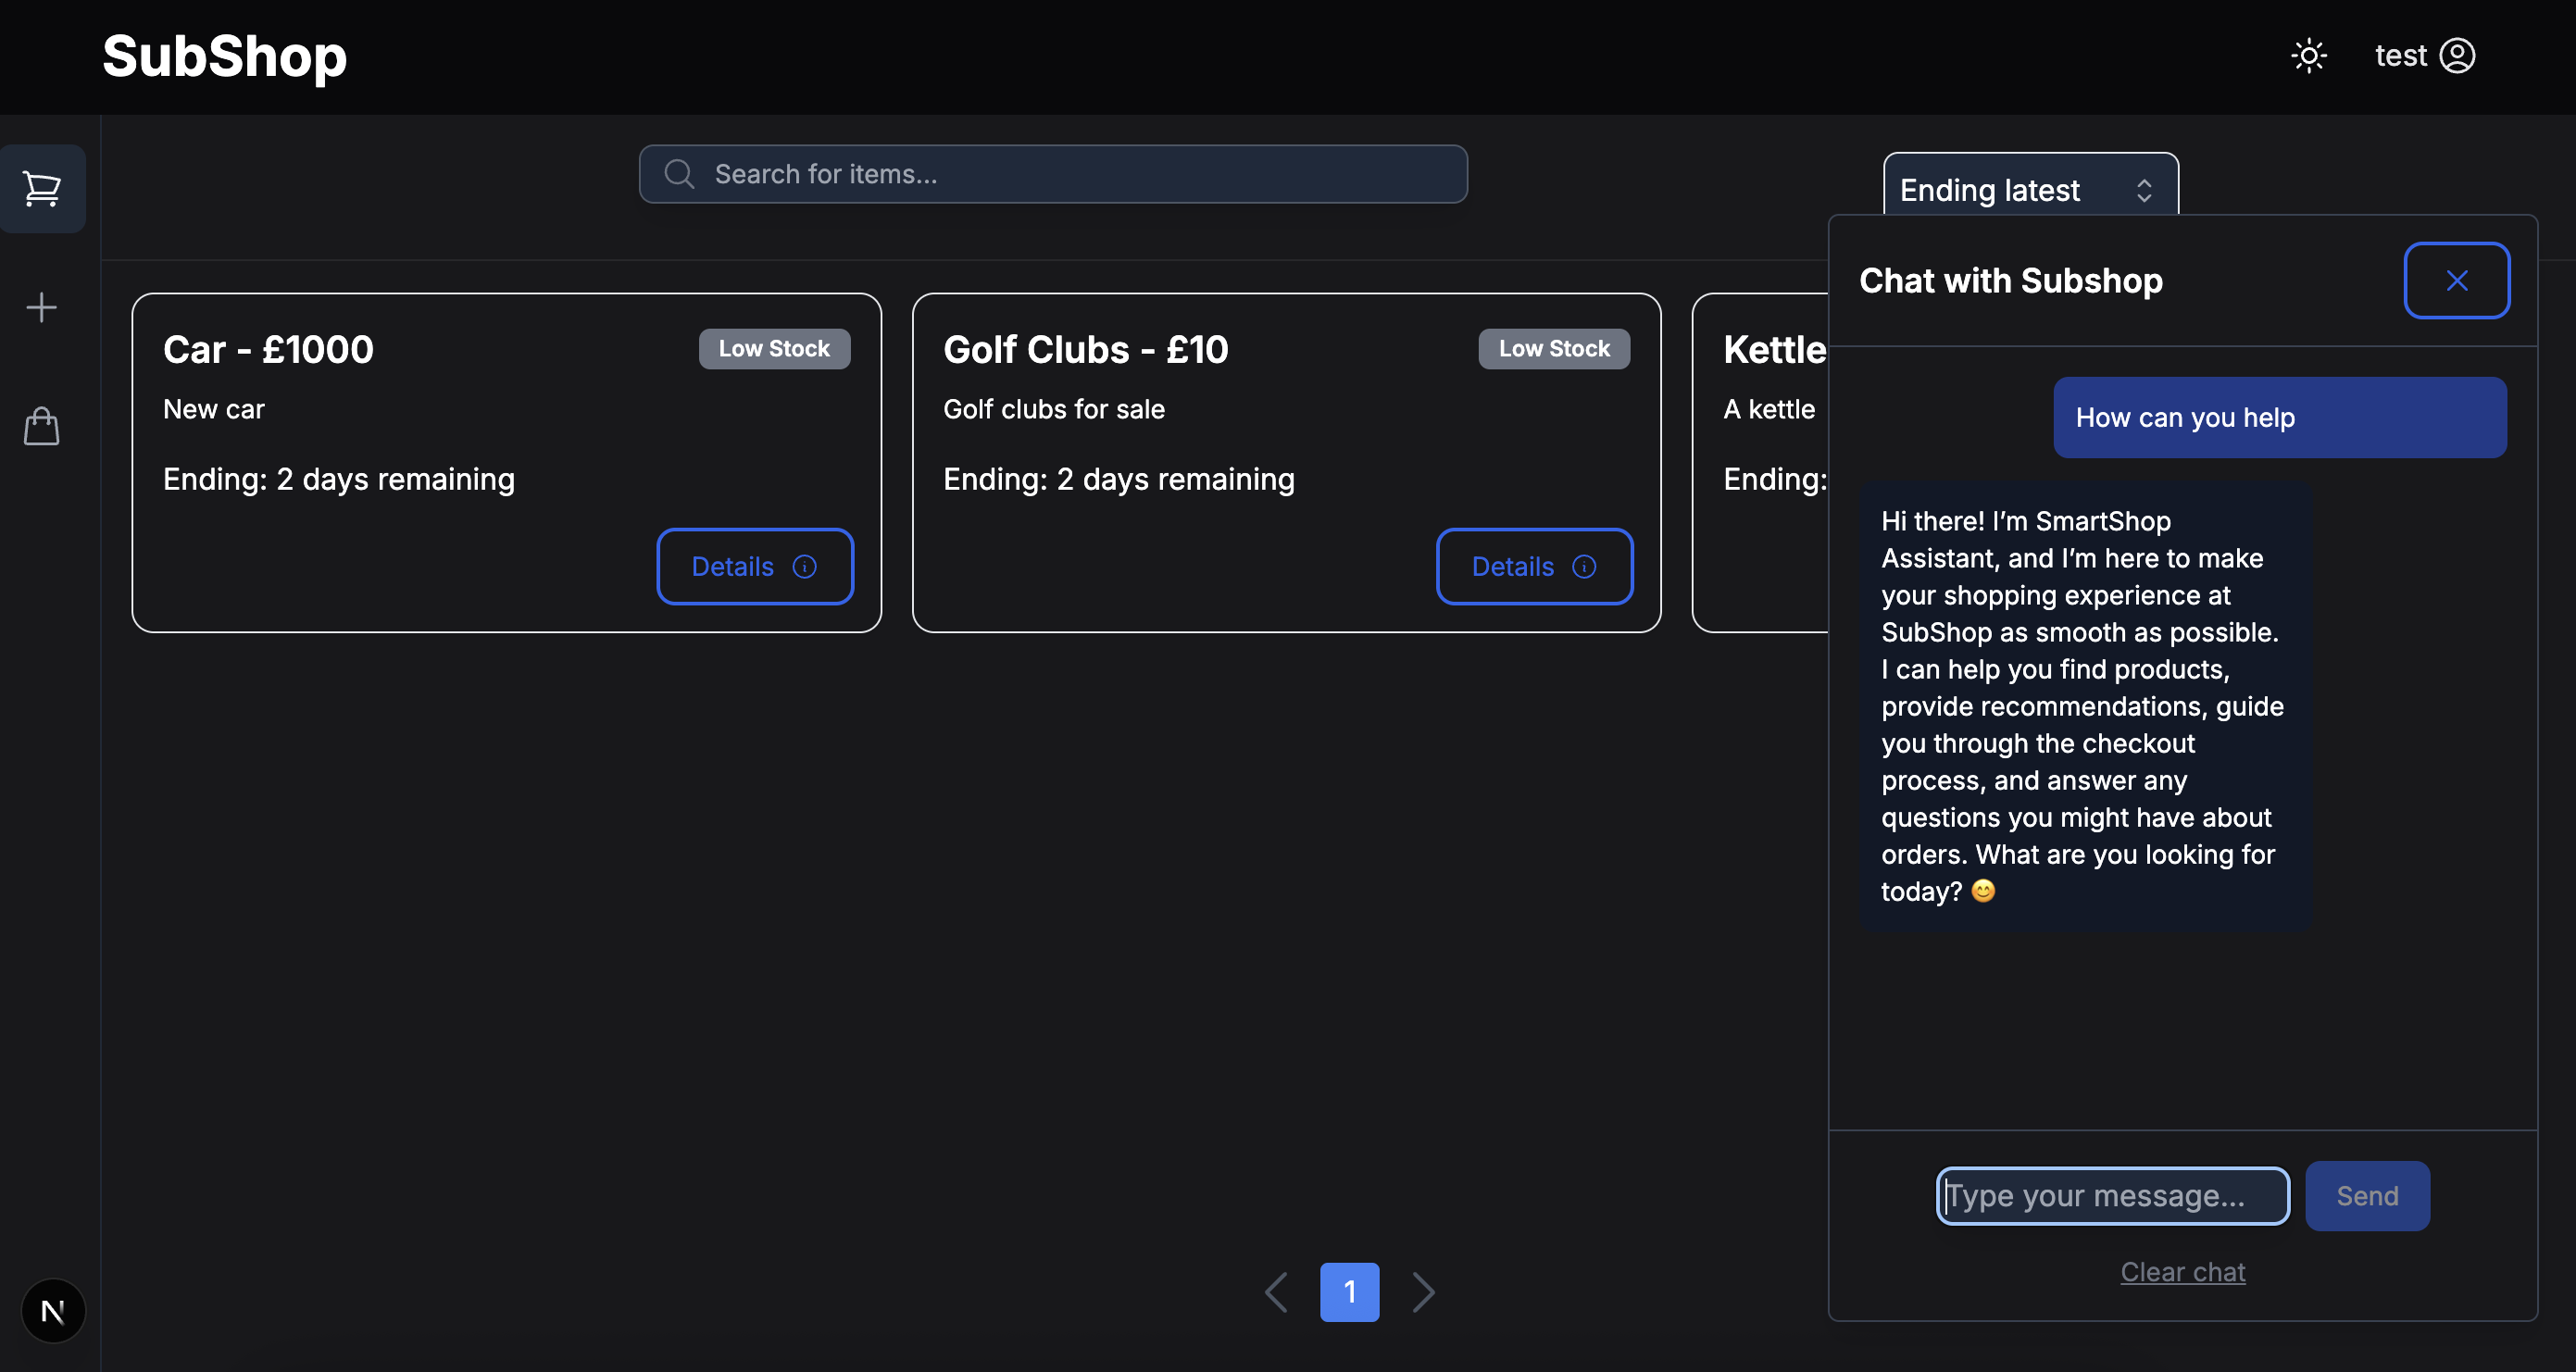
\includegraphics[width=\textwidth]{Shop.png}

If you see an item that you might be interested in you can press the details button which shows more information about an Item as well as allows you to bid against other people for the item. The payments here do not take any money they just authorise the funds being taken once the auction is finished.

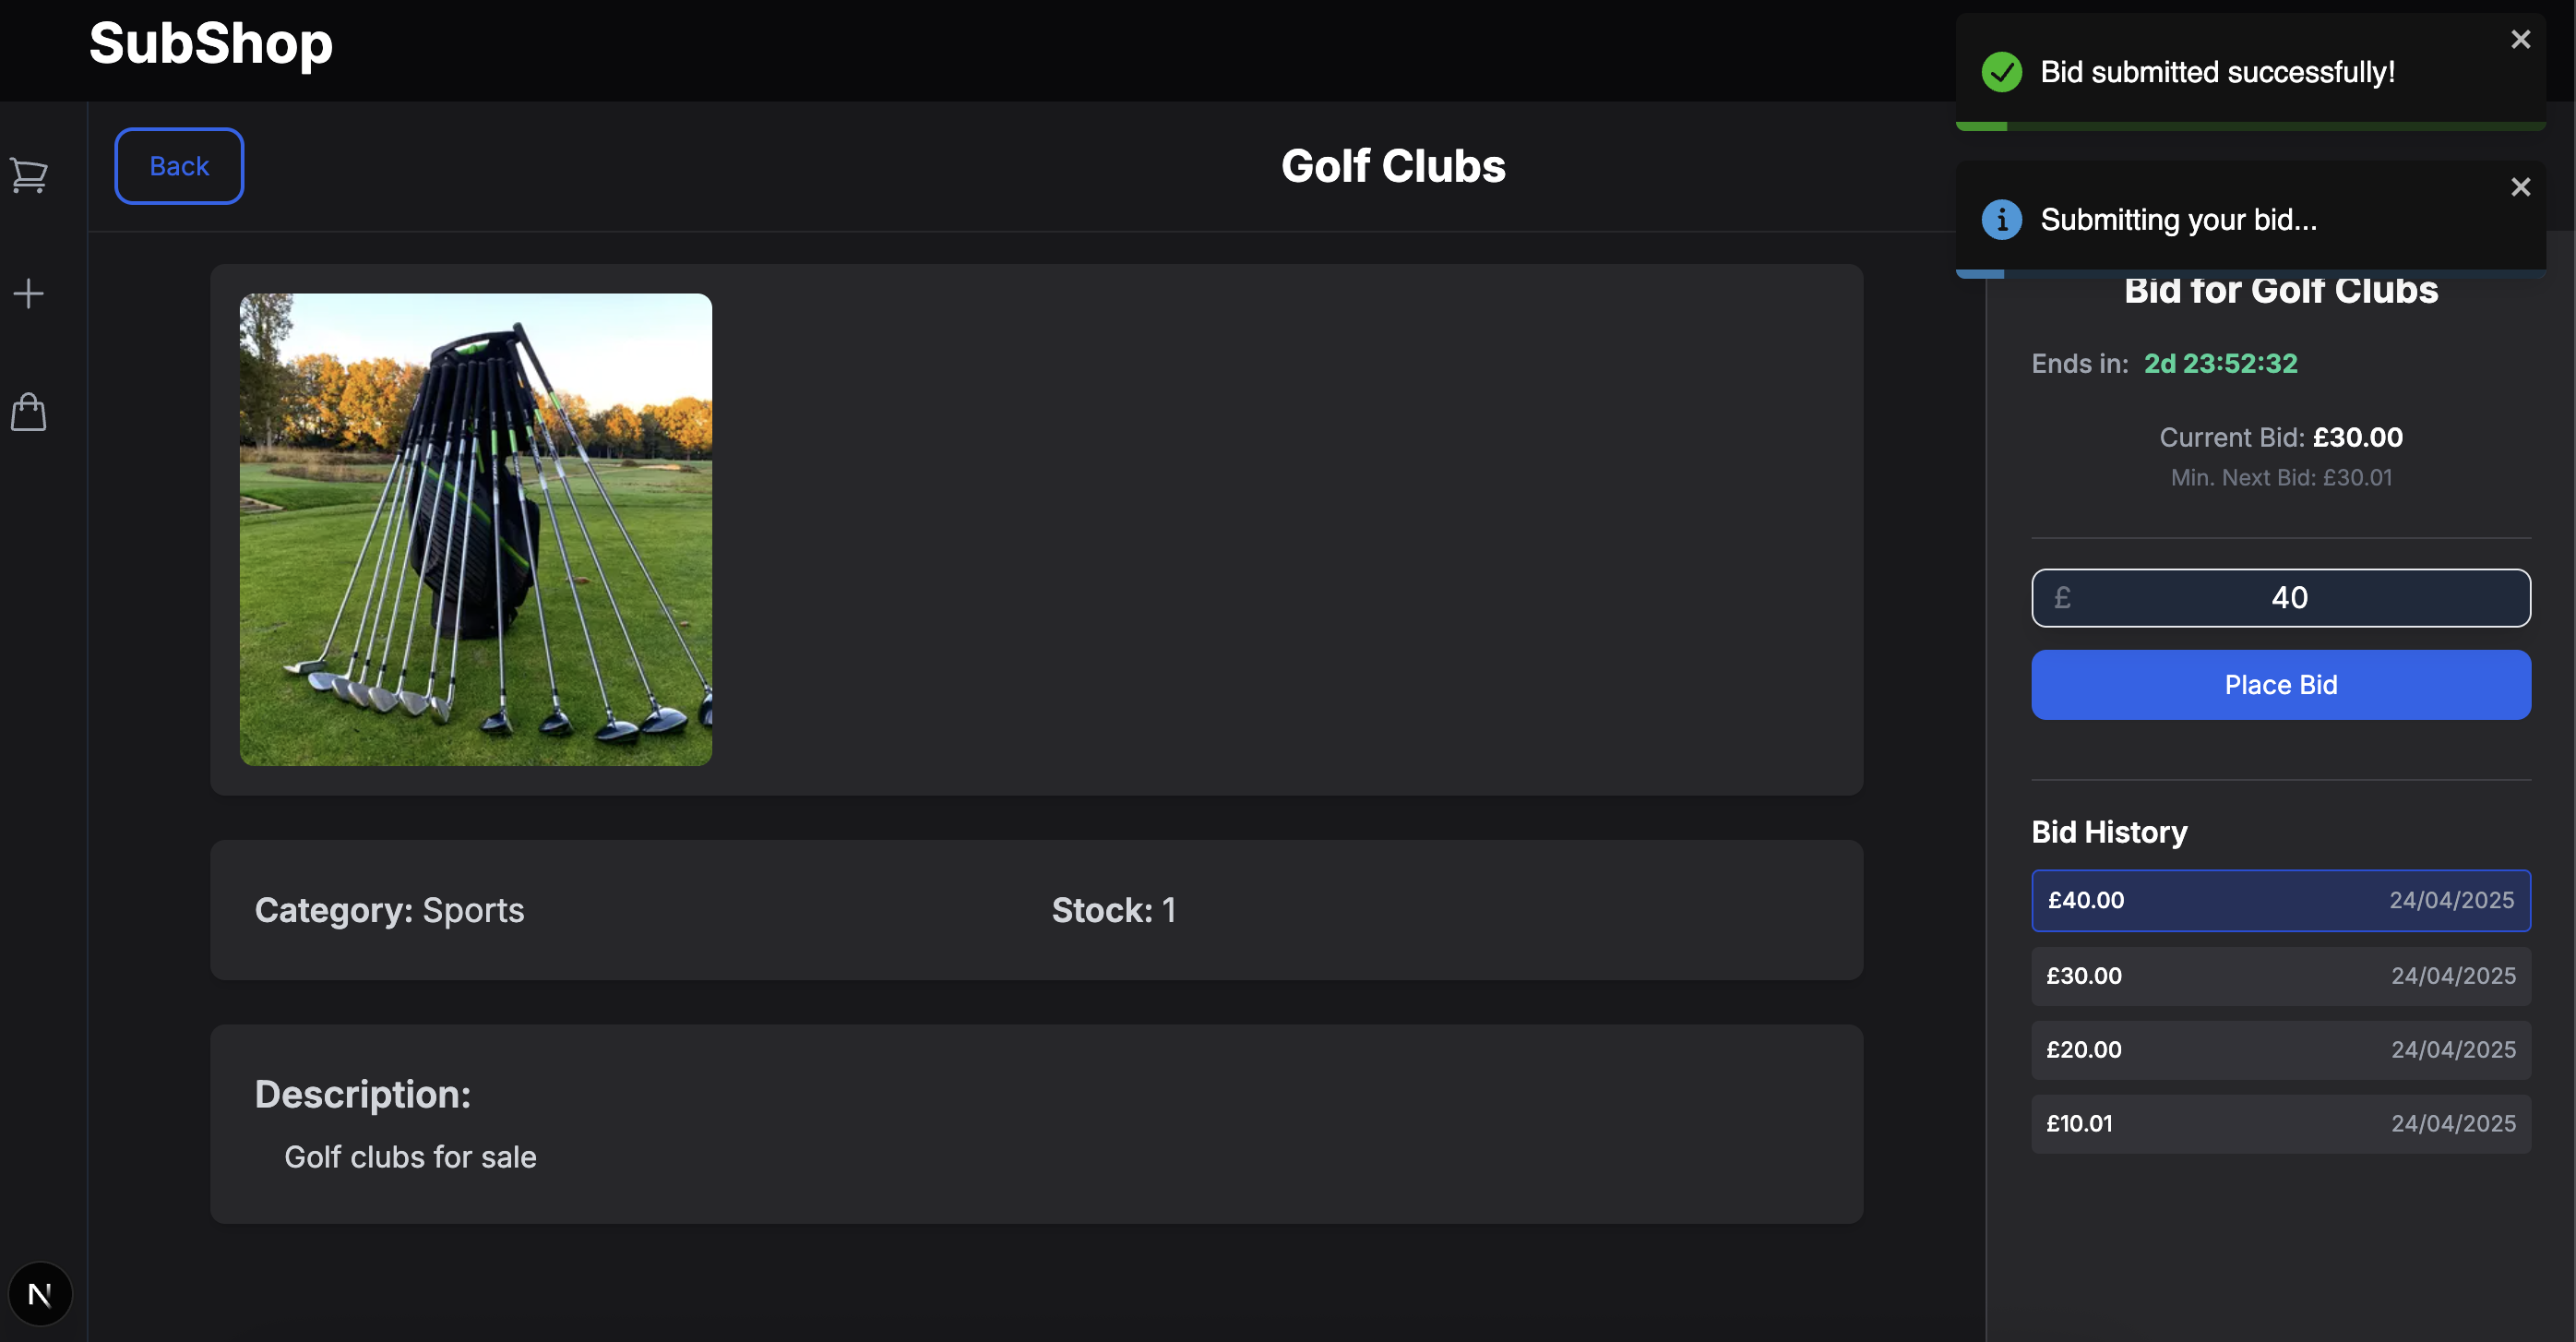
\includegraphics[width=\textwidth]{ItemPage.png}

Finally, if you win the auction, the payment will go through and the item will be sent to your account. 


\subsection{Admin Use}
To create the first admin you need to add the Cognito Group to the specific user and update the database admins table manually, after that you can use the admins dashboard shown below to promote users to admins and assign them permissions. As well as that if you have the correct permissions then you can view all of the admins, users and permissions.

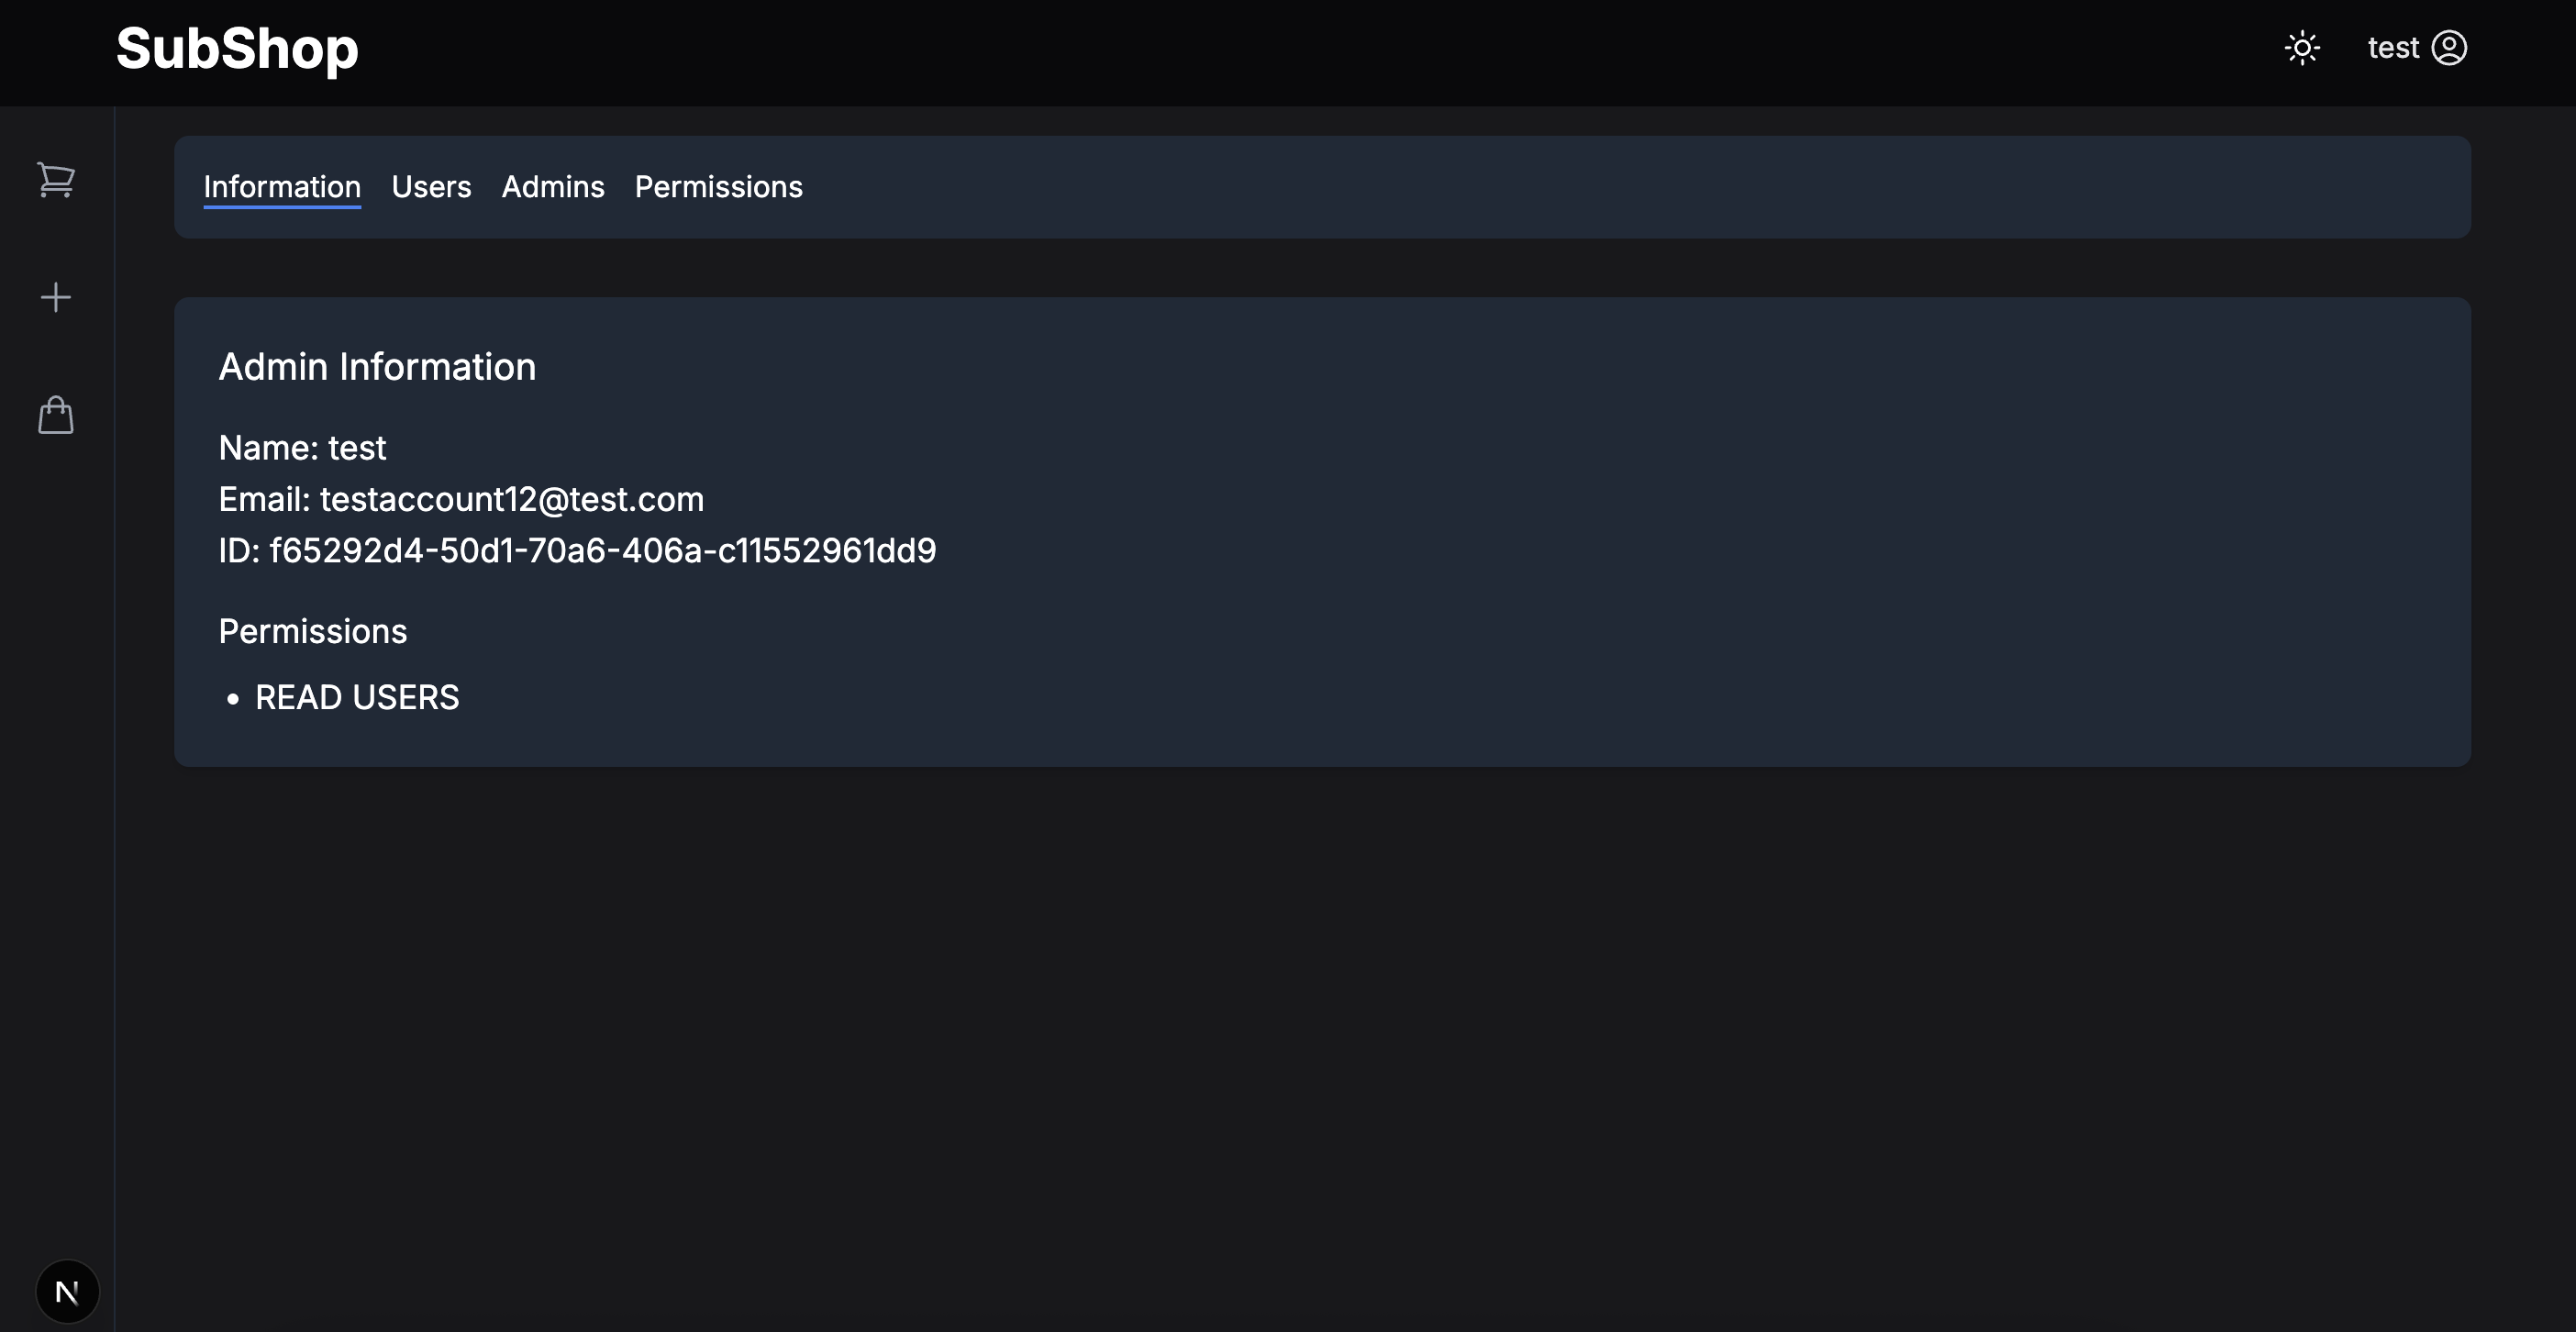
\includegraphics[width=\textwidth]{AdminPage.png}



\chapter{Reflection}
Overall the project progression was very good but there were some things that need to be reflected on. Firstly, while the harder features such as cloud deployment, CI/CD and event driven architecture with streaming are important, they did slow down progression as they were new technologies to learn so they did require more time to develop, this meant that some other features were missing important features such as the logins error handling. 

Secondly, as discussed in the testing section above, the frontend and integration tests were slightly neglected as development speed was a priority so it was harder to keep these all updated.

Different subscriptions with different tiers weren't added and this was one of the main features that was wanted, although all of the supporting features were almost completed so it would not be too hard to add in this feature.

The handling of items after auctions has not been fully completed and there is no setup for the postage of items has not been setup or implemented.

While the backend was created in one service, which at the time was great, there are plans to separate it into smaller, independent services that can utilise the gateway and create a GraphQL Federation. This will have great benefits but the initial creation of it as one service was the right idea.

Finally, the diary inside the git repository was not updated as regularly as it should have been, while the progress was tracked in separate documents, it was not frequently updated inside the git repository and it would have been better to do so.

\chapter{Future plans}
The first things to be done would be to go over the reflection and try to resolve what was found there, then the plan is to break the code up into separate services and potentially repositories so that it is easier to onboard developers and maintain the code. As this all was made with a tight deadline it will be important to take a step back and try and find any mistakes made during development. Finally, reaching out to users and trying to gain traction, improve the application based on their needs and wants as well as continued feature development.

\bibliographystyle{ieeetr}
\bibliography{final-report}
\addcontentsline{toc}{chapter}{Bibliography}

\chapter*{Appendix}
\addcontentsline{toc}{chapter}{Appendix}


\appendix

\chapter{Diary}

\section{Week 1}
\begin{itemize}
    \item I met with my supervisor to discuss what the project entails and to also discuss my initial plan.
    \item I am struggling to decide on what product I want to build but I am thinking about creating a store application that allows for individual users, teams and enterprise users.
    \item I have been researching technologies that I am planning on using both now and In the future.
    \item After researching the technologies I wanted to use I found some issues with how to test them so I am evaluating what would be the best option, I also asked my supervisor what they thought would be a good approach, with the advice I got and the research I completed I will be able to narrow down what to use.
    \item Finally I have been working on my project plan and have started the abstract, created an initial timeline and started thinking about the risks my project has.
\end{itemize}

\section{Week 2}
\begin{itemize}
    \item I continued working on my project plan, I had some areas where I was unsure so I asked my supervisor to read over one of my drafts.
    \item I continued to research web technologies and I am planning on setting up the initial application.
    \item I updated my plan based on the recommendations I received and finished it off.
    \item I submitted the project plan and merged it into the \texttt{main} branch of this repo as well as creating a tag for it so that I can easily track when it was completed.
    \item I had planned on setting up the initial application and I will have some of it set up but it will be hard to fully understand the requirements until my project plan has been marked and I have some feedback on it.
\end{itemize}

\section{Week 3}
\begin{itemize}
    \item I spent the majority of this week planning and researching.
    \item I have decided to use a \texttt{Java Spring Boot} application with a \texttt{PostgreSQL} database for the backend and a \texttt{Typescript Next.js} Frontend.
    \item I created an inital setup for both the frontend and backend and I plan to continue working on the setup over the next week.
    \item I did lots of research on all of these frameworks as well as authentication providers and payment providers.
\end{itemize}

\section{Week 4}
\begin{itemize}
    \item I setup the authentication provider that I am planning to use. To do this I used the research I did on \texttt{AWS Cognito} and \texttt{Terraform} so that I could provision it using Infrastructure as Code (\texttt{IaC}).
    \item I also setup \texttt{Apollo Client} on the frontend which I will use to manage the states of my data and interact with the backend of the application.
    \item Finally I setup \texttt{GraphQL Codegen} which will enable me to generate type safe code from my \texttt{GraphQL} schema.
\end{itemize}

\section{Week 5}
\begin{itemize}
    \item I setup authentication on the frontend which now allows for a user to login if they have a \texttt{Cognito} user account.
    \item I then setup the use of \texttt{JWT} for authorisation. This was only setup to send the \texttt{JWT} to the backend.
    \item I started adding \texttt{JWT} verification on the backend but I started getting lots of issues with \texttt{CORS} once I added \texttt{Spring Security}. This meant that the issue is rolling over into Week 6.
\end{itemize}

\section{Week 6}
\begin{itemize}
    \item I met with my supervisor this week and discussed my current progress, I identified that I need to start my reports as soon as possible so I am planning on doing that.
    \item I finished off the initial backend security that I was working on and merged it.
    \item I have been building the user interface out.
    \item Created different security profiles for the backend.
    \item I created a database and an initial users table in it.
\end{itemize}

\section{Week 7}
\begin{itemize}
    \item Created unit and integration tests for the backend.
    \item Added \texttt{Checkstyle} to the backend and fixed existing issues.
    \item Started to create \texttt{GitLab CI} pipelines for the project.
    \item Started my interim report.
\end{itemize}

\section{Week 8}
\begin{itemize}
    \item Continued to work on the pipelines but had lots of issues with the images they would run on.
    \item Added a \texttt{userDetails} table which contained basic information about a user.
    \item Created the UI for the user details.
    \item Researched \texttt{Netflix DGS} to fix errors and created custom datafetchers for the user details.
\end{itemize}

\section{Week 9}
\begin{itemize}
    \item Finalised the user details UI, backend and the database schema and functions.
    \item I updated the security config, specifically the \texttt{JWT} decoder.
    \item Fixed the backend pipeline as the new changes were causing errors.
    \item Continued to work on my interim report.
\end{itemize}

\section{Week 10}
\begin{itemize}
    \item I added items to the database and backend.
    \item I setup initial searching of the items.
    \item Created and completed the presentation slides for week 11.
    \item I added end-to-end and component testing to the frontend.
    \item Added and configured \texttt{Knip} for the frontend.
\end{itemize}

\section{Week 11}
\begin{itemize}
    \item Updated the frontend security info.
    \item Setup initial \texttt{Stripe} subscriptions.
    \item Added steps to setup the \texttt{Stripe} subscriptions.
    \item Presented my presentation and watched peer presentations.
    \item Finished the interim report.
\end{itemize}

\section{Week 12}
\begin{itemize}
    \item Assessed status of project and made a plan on what to do going forward.
    \item Created SQL tests for the database.
    \item Setup \texttt{Redis} as a cache.
    \item Setup Cache connection from backend.
    \item Implemented initial caching with \texttt{Redis}.
    \item Setup \texttt{Cognito} in the integration tests.
\end{itemize}

\section{Week 13}
\begin{itemize}
    \item Setup a delete user functionality that soft deletes users so that some important information is not lost.
    \item Started to work on the AWS infrastructure.
    \item Changed the setup of the \texttt{IaC}.
\end{itemize}

\section{Week 14}
\begin{itemize}
    \item There was lots of progress with the infrastructure this week but it was all works in progress so there is not much in the diary.
\end{itemize}

\section{Week 15}
\begin{itemize}
    \item The infrastructure overhaul was completed this week but there are still things to work on with it.
    \item A production merge was made after configuring the code for it.
    \item The User interface for searching was created and the implementation was started.
\end{itemize}

\section{Week 16}
\begin{itemize}
    \item There was more infrastructure overhaul this week as the load balancers were setup and \texttt{SSL}.
    \item Work on \texttt{SES} (Simple Email Service) and the implementation was started here and hoping to be completed by the end of the week.
\end{itemize}

\section{Week 17}
\begin{itemize}
    \item The \texttt{SES} infrastructure and implementation were completed like planned.
    \item An integration with \texttt{Jira} for bug reporting was created.
    \item A backend logging solution was added.
    \item Fixes for the integration tests were completed.
\end{itemize}

\section{Week 18}
\begin{itemize}
    \item Started the final report.
    \item Lots of new backend features were created this week.
    \item Queries and mutations for items were made.
    \item Pagination was added and worked on.
    \item The create item UI was made.
\end{itemize}

\section{Week 19}
\begin{itemize}
    \item Queries to get items by users were made.
    \item The backend was restructured and refactored.
    \item The \texttt{GraphQL} schema was restructured as well.
    \item Pages for the users items were created.
    \item A production merge was made.
\end{itemize}

\section{Week 20}
\begin{itemize}
    \item Frontend pagination, sorting and filtering were added where possible.
    \item The shops items got an overhaul.
    \item Admin features were started to be worked on.
\end{itemize}

\section{Week 21}
\begin{itemize}
    \item Admin features were created and worked on heavily.
    \item There were lots of fixes to do with the admins.
    \item Especially to do with how the caching worked here.
    \item Production merge.
\end{itemize}

\section{Week 22}
\begin{itemize}
    \item More infrastructure updates.
    \item This mainly was to do with the \texttt{CI/CD}.
    \item Test, build and deployment stages were created inside a pipeline.
\end{itemize}

\section{Week 23}
\begin{itemize}
    \item An integration with \texttt{OpenAI} was started.
    \item A AI chatbot was added.
    \item Work for an \texttt{Apollo Gateway} was started.
\end{itemize}

\section{Week 24}
\begin{itemize}
    \item There were lots of updates to the gateway and it was completed.
    \item But it was parked for now as the backend is still one service.
    \item The infrastructure was also setup and parked.
\end{itemize}

\section{Week 25}
\begin{itemize}
    \item The bidding service was setup and completed.
    \item \texttt{Kafka} was configured and added.
    \item Final infrastructure updates were made.
    \item The final changes were added.
    \item The final report was finished.
\end{itemize}

\end{document}